\chapter{User centered design}
Many projects are developed based solely on the idea of a person or a group of people, who are sure that there is a group of people who feel the same way about the project. They invest time and resources in developing the product they imagine, but when they launch said product they find that they might have overestimated the amount of people that would be interested, that the very clear, intuitive and useful features turned out to actually be confusing, saturated and not very useful for most users. Many projects suffer unexpected problems when they are released, because they are developed in a vacuum, completely removed from potential future users and following only what the team believes and assumes is intuitive and useful.\\
Including the people who are expected to use the software in the conception of the tool itself causes, on one hand, the complexity to grow rapidly, given that the feedback from those users must be now taken into account and said feedback con sometimes be at odds with what the development team had in mind, thus complicating the decision making and development processes. But on the other hand, this increased complexity brings a great added value into the project, by avoiding or at least greatly reducing possible surprises at launch.  The tool can be developed knowing that there is a group of people interested in it, who have the same, or very similar ideas, desires, habits, etc., to those which the team had in mind and intended to address. This means, that nothing is not being developed for a group of imaginary people with fabricated desires and needs.\\
For this project in particular, different tools where used to contact potential future users and gather information about their desires, ideas, habits, etc., regarding keeping track of pending tasks: The first step was carrying out a focus group to gain an initial of the space. After this and based on the results, a survey was conducted to gain further insights and identify where the participants' interests lay. Lastly, a paper prototype was developed in order to perform a set of heuristic evaluations to find possible usability issues and refining the idea before starting the implementation. The implementation and results of these procedures will be presented in the following chapter. Due to the iterative nature of the user-centered design process, it is always possible to conduct more studies, interviews, etc., but given the strict time constraints present in this project, an itinerary was defined which would, on one hand, would allow to take full advantage of the user-centered design process and get as much information as possible, while also leaving enough time available for the other aspects of the project.

\section{Focus Group}
As mentioned before, the first step in the project was to conduct a focus group. This interview marked the beginning of the first phase of the user-centered design process, namely the analysis and description of the use context \cite{usabilityUXBook}. The focus group was conducted with the idea of serving as a first approach towards potential users, to create a general idea of the area and its users and to begin to understand the use context. This initial approach served as a guide to define in which direction the project should move next. \\

\subsection{Participants}
Eight participants took part in the focus group: five women and three men, all between the ages of 21 and 25 who were either university students with a job or recent graduates of the past two years. The composition of this group is due to the fact that, even though the final application was developed with the intention that it could be used by everyone and did not require any special skills or knowledge, this first approach had to provide as much information as possible, since it would be the basis for many important decisions regarding the next steps of the project. For this reason, it was not only necessary to ensure that the participants all had a lot to say on the subject, but also that they were comfortable using digital tools and voluntarily chose them to solve or alleviate areas of their daily lives (even if not specifically in the area of managing and organizing pending tasks), because if these characteristics were met it was more likely that they would be open to adopting software or an app to organize their daily lives. Given these requirements and the fact that this project was developed in an academic context, it was very likely that university students or recent graduates would meet these requirements. In addition, interviewing people who had a job and were or were students had another positive aspect, which was that it was naturally beneficial if the participants had already dealt with the topic a bit more in depth before the focus group, something that many students must do to prepare themselves for their studies and their subsequent or parallel jobs.

\subsection{Medium and Procedure}
%TODO Add focus group duration
The interview was conducted virtually, via a group video call and with the help of a virtual whiteboard, which lasted about . It was not carried out in person to facilitate the planning and execution of the event, as scheduling the availability of 8 people in completely different contexts and with completely different agendas is not a simple task and the interview had to be carried out promptly. The use of the virtual whiteboard was of vital importance, since it allowed the participants to work collaboratively and visually, a central factor of focus groups as it fosters creativity and idea generation. With the help of this tool, the process of a face-to-face focus group could be effectively simulated by allowing participants to place virtual sticky notes on top of a whiteboard prepared by the moderator and the use of shapes and text to create new elements (see \ref{}). \\
The interview was conducted in English, as this was the language that all participants shared and in which most were comfortable. First, a formal introduction was given, explaining the logistics and how the focus group would be carried out as well as the motivation and purpose  the focus group and the project as a whole. It was explained to the participants that the goal was to get an insight into how and why (or why not) they planned their tasks and if there were any pain points or highlights in terms of task tracking. After this, the participants answered and discussed several questions, described in the following section.

%La entrevista se llevo a cabo de manera virtual, mediante una video llamada grupal y con la ayuda de un whiteboard virtual. No se hizo en persona para facilitar la planeacion y ejecucion del evento, debido a que organizar la disponibilidad de 8 personas en contextos y con horarios completamente diferentes no es una tarea simple y la entrevista se debia realizar con rapidez. El uso del whiteboard virtual era de vital importancia, debido a que permitia a los participantes trabajar de manera colaborativa y visual, un factor central de los focus groups ya que fomenta la creatividad y la generacion de ideas \cite{}. Con ayuda de esta herramienta se podia simular el proceso de una focus group presencial de manera efectiva, ya que permitia a los participantes colocar notas adhesivas virtuales encima de una pizarra preparada por el moderador y utilizar formas y texto para crear nuevos elementos (see \ref{}). \\
%La entrevista se llevo a cabo en ingles, debido a que era el idioma que todos los participantes compartian y en el que la mayoria se sentia comodo. Primero se hizo una introduccion tanto formal, sobre la logistica y como se iba a llevar a cabo el focus group como sobre el contenido y proposito del trabajo y del focus group. Se les explico que la meta era get an insight into como y por que o por que no organizaban sus tareas como tambien sobre posibles pain points o highlights en cuanto a la tracking de actividades. Luego de esto, los participantes respondieron y discutieron las preguntas, descritas en la siguiente seccion. En total el focus group duro .
%ADD TIME 

\subsection{Tasks}
El focus group se dividio en tres tareas. Cada una buscaba, utilizando diferentes metodologias, analizar y ahondar en aspectos diferentes de las rutinas, costumbres, comportamientos, expectativas, problemas, etc., de los participantes:

\myparagraph{Description of personal habits and routines}
El objetivo de esta primera pregunta era por un lado recopilar informacion sobre los habitos de los participantes en cuanto al seguimiento de tareas pendientes y por el otro lado estimular a los participantes para que analizaran sus procesos de manera consciente. Dependiendo de si los participantes mantenian un registro o no, debian responder un conjunto de preguntas diferentes.
En caso de que la respuesta fuera afirmativa, los participantes debian responder las siguientes preguntas:

\begin{enumerate}
    \item How often they tracked and managed their pending tasks and if they had a routine.
    \item Where they kept track of their tasks (PC, smartphone and/or paper).
    \item If and which tools they used (digital and analog) to keep track and manage their tasks.
    \item To describe in detail their individual process of writing down and keeping track of tasks.
\end{enumerate}

En caso de que la respuesta fuera negativa, las preguntas que debian responder los participantes eran las siguientes:

\begin{enumerate}
    \item What was the reason for not keeping track of their pending tasks.
    \item How they usually kept an overview of pending tasks.
    \item How they made sure to not forget to complete their pending tasks.
    \item If there was something that could make them start keeping track of their pending tasks.
\end{enumerate}

Para esta pregunta, a los participantes se les dieron aprox. 10 min. para que respondieran por su cuenta. Durante este tiempo, el moderador fue agrupando las respuestas iguales o similares para crear clusters.  Luego los proximos 20 min. se utilizaron para, con la ayuda del moderador, discutir a fondo todas las respuestas y dar la oportunidad a todos los participantes de explicar sus procesos y los razonamientos subyacentes. La utilizacion de estos bloques de tiempo pretendia dar a los participantes tiempo donde se pudieran concentrar y analizar la pregunta a fondo, pero que tambien tuvieran un espacio para discutir y explicar sus puntos.\\
\\
De los 8 participantes no habia ninguno que no mantuviera un registro de sus tareas pendientes, por lo que no hubo respuestas para las preguntas del caso negativo. \\
En cuanto al caso positivo, 6 reportaron que revisaban y actualizaban sus tareas de manera diaria, un participante agrego que si sabia de tareas en los proximos dias o semanas, tambien los incluia y otro dos especificaron que esto solo incluia tareas del trabajo ya que no mantenian un registro para tareas personales. Los otros dos participantes organizaban sus tareas pero de maner irregular y sin rutina especifica. Uno de ellos los actualizaba de manera semanal y el otro no tenian ningun tipo de intervalo fijo.\\
En cuanto a donde mantenian sus tareas, la mayoria de los participantes utilizaban diferentes metodos para organizar diferentes tareas. La mayoria, es decir seis partucipantes, lo hacia en su smartphone, seguido de cerca por un empate entre la PC y el papel, ambos utilizados por 5 participantes. Concretamente, de los 5 participantes que utilizaban papel, cuatro utilizaban una agenda o un cuaderno, dos utilizaban notas adhesivas y uno utilizaba un calendario de papel. En cuanto al motivo por el que utilizaban papel, 4 de los 5 participantes estaban de acuerdo en que les gustaba el sentimiento tactil que brindaba el papel y que el sentimiento de tachar tareas completadas era satisfacotorio y los hacia sentir mas productivos. Un participante comento ademas, que le gustaba el hecho de que el papel solo tuviera un posible uso, a diferencia del PC o el smartphone, lo cual lo ayudaba a no distraerse y mantenerse productivo. 
\\
\\
La herramienta mas utilizada por los participantes fue el calendario digital, concretamente Apple y Google Calendar, utilizada por 4 participantes, de los cuales dos senalaron que utilizaban esta herramienta unciamente para registrar eventos con fecha y posiblemente hora.\\
En el segundo puesto en cuanto a cantidad de usuarios hubo un empate entre los simple task managers (concretamente Google Keep y Apple Reminders), project management software (especificamente Jira y Windows Planner) y la native note-taking software (concretamente las aplicaciones ofrecidas por Apple, Windows y Android), cada un con 3 participantes que los utilizaban. En relacion a los simple task managers un usuario especifico que los utilizaba debido a que le permitian poner reminders y notificaciones a sus tareas y otra participante menciono que solo lo utilizaba al viajar pero por el mismo motivo. De los tres participantes que reportaron el uso de project management software, solo uno lo utilizaba de manera privada mientras que los otros dos lo utilizaban en el trabajo y no de manera voluntaria. Un participante noto ademas que saltaba entre project management software y las native note-taking software de Windows y de Android, y que aparte de cual tenia mas a la mano en el momento y era la mas rapida de abrir, no habia ningun otro motivo concreto en cuanto al momento de decidir que aplicacion iba a utilizar. \\
Un unico participante respondio que utilizaba un documento de texto simple para anotar y organizar sus tareas y que imprimia sus calendarios para tenerlos en un formato fisico, ya que ambos metodos le brindaban soluciones simples, de rapido acceso y con un buen overview.\\
Por ultimo, un participante dijo que para el trabajo ocasionalmente utilizaba una highly customizable general purpose applications, concretamente OneNote, debido a que esta era la aplicacion que mas se parecia a la agenda fisica que utilizaba regularmente, al ofrecer un lienzo en blanco sin ninguna estructura concreta.
\\
\\
Cuando se les pidio a los participantes que describieran su proceso usual de anotar, organizar y actualizar sus tareas, cada participante describio procesos diferentes y tailored a sus necesidades:\\
El participante que utilizaba el documento de texto simple y el calendario impreso, describio su proceso como una estructuracion muy general por categoria, que usualmente son sus proyectos, pero con un proceso constantemente cambiante y que se apega a las necesidades actuales.
El segundo participante anotaba las tareas mas importantes en su smartphone en el calendario digital de Apple y les ponia un reminder para que no se le pudiera olvidar. Las tareas menos importantes las anotaba cada una en una nota adhesiva que luego colocaba sobre su escritorio para siempre tenerlos a la vista y los revisaba diariamente.\\
El tercer participante tenia dos rutinas diferentes, dependiendo de su entorno: Si se encontraba en el trabajo, utilizaba un sistema de tickets en un project management software (Jira), impuesto por la compania, donde cada ticket contenia una tarea, la persona responsable, el tiempo estimado de realizacion y la fecha de entrega. En su vida privada, utilizaba un cuaderno donde anotaba todas las tareas que debia completar ordenadas por prioridad y a medida que las iba completando las iba tachando de la lista.
El cuarto participante anotaba y organizaba principalmente sus tareas laborales escribiendolas en un cuaderno. Iniciaba primero escribiendo todas las tareas generales que debia completar y luego especificaba para cada tarea general todas las sub tareas mas especificas.\\
El quinto participante, el cual saltaba entre project management software y las native note-taking apps de Windows y Android, no tenia una estrategia concreta aparte de simplemente organizar su lista por prioridad e iba adaptando su estrategia on the fly, cambiando de una a otra aplicacion dependiendo de cual tuviera a la mano mas rapido y apegando su estrategia de organizacion a lo que necesitara en el momento. Lo que si era importante para este participante era que al completar las tareas no las tachara y permanecieran en la lista, sino que las borrara permamentemente, para mejorar su overview de las tareas restantes.\\
De igual manera que el cuarto participante, el sexto participante tambien organizaba unicamente sus tareas laborales, para las privadas utilizaba unicamente su memoria. En el trabajo regularmente tenia sesiones de planificacion, donde todos los participantes discutian sus tareas y organizaban sus calendarios correspondientemente, donde el participante especificamente utilizaba un calendario digital. 
El septimo participante anotaba y organizaba sus tareas para toda la semana en una agenda. Si las tareas tenian hora y fecha eran escritas bajo el dia y hora correctos y si no, eran anotados en una lista sin ningun tipo de orden y las tareas mas importantes eran resaltadas con un resaltador. El participante revisaba y actualizaba su agenda y las tareas de manera diaria.\\
Por ultimo, el ocatvo participante escribia de manera diaria todas las tareas que le vinieran a la mente en un cuaderno ordenadas por prioridad. Si se le ocurrian otras tareas durante el dia, las registraba en su smartphone con la ayuda de un simple task manager, concretamente Apple Reminders, para poder agregar notificaciones y fechas de entrega a las tareas.

\myparagraph{Description of ideal too}
En la segunda pregunta, a los participantes se les pidio que se imaginaran que tenian la oportunidad de disenar y desarrollar un sistema para organizar sus tareas pendientes. Solo tomando en cuenta sus necesidades, deseos y pain points personales, se les pidio que anotaran todos los puntos que se les ocurrieran sobre los tres proximos puntos:

\begin{enumerate}
    \item Which features and characteristics would be required to be included, both functional and aesthetic.
    \item Which features and characteristics would be welcomed but not required to be included, both functional and aesthetic.
    \item Which features and characteristics could under no circumstances be included, both functional and aesthetic.
\end{enumerate}

Con esta pregunta se pretendia entender que funcionalidades eran consideradas utiles o inutiles y positivas o negativas por los participantes. De esta manera se creaba una primera pequena coleccion de features que se podian seguir analizando en los proximos pasos del proyecto. \\ 
El proceso de esta pregunta fue iqual que el de la anterior: Los participantes primero anotaron sus respuestas por su cuenta y luego se abrio el espacio para que discutieran sus respuestas.\\
\\
En esta seccion, como mencionado anteriormente, se pidio a los participantes que se imaginaran que debian desarrollar una aplicacion para organizar tareas pendientes y que recolectaran todos los features y caracteristicas que se les ocurrieran para cada categoria presentada. \\
\\
Los resultados para la primera categoria, que eran los aspectos que de ninguna manera podian faltar en su aplicacion imaginada, estan resumidos en la tabla \ref{tab:reqFeaturesTable}. En dicha tabla se puede apreciar, que hubo muchas ideas que resonaron con los participantes y con las que estuvieron de acuerdo, siendo la primera que la aplicacion debia ofrecer cross-platform, es decir poderse usar en diferentes tipos de hardware, principalmente PC y smartphone. Esta necesidad se puede ver reflejada en las respuestas anteriores, donde muchos participantes utilizaban mas de una herramienta dependiendo de que tipo de hardware estuvieran utilizando y en que situacion se encontraran. \\
Cuatro participantes opinaron que la aplicacion debia ofrecer diferentes vistas para visualizar las tareas pendientes, p.ej. calendario y lista. El deseo por este feature puede leerse entre las líneas de las respuestas anteriores, donde varios participantes reportaron que utilizaban simultaneamente calendarios digitales para organizar tareas que tuvieran una fecha limite y otras herramientas para tareas sin fecha de entrega.\\
Otro tema importante que se vio reflejado en las respuestas de los participantes es que no solo los features independientes de la aplicacion deben ayudarlos con sus tareas, sino que en general la aplicacion debia ser facil de usar y entender, presentando un diseno que no solo fuera muy simple y que brindara claridad sobre su funcion sino que tambien hiciera que la aplicacion fuera visualmente atractiva. Es decir, que para los participantes era importante que la aplicacion no solo les brindara features para ser mas eficientes y organizar sus tareas pendientes, sino que el diseno de la aplicacion como tal tambien los apoyara en este punto, ofreciendo una combinacion entre funcionalidades robustas y un diseno que por un lado sea simple, claro y que no abrume al usuario y que por el otro lado sea atractivo visualmente y le cause gusto al usuario utilizar la aplicacion. 
%TODO Investigar sobre visualmente atractivo = Mas ganas de usar aplicacion
\\
Otro punto importante para los participantes era la capacidad de tachar tareas una vez completadas, aspecto que tambien fue mencionado en las preguntas anteriores. Los participantes mencionaron que les daba satisfaccion tachar las tareas, debido a que esto significaba que la habian completado, sino que tambien les daba satisfaccion ver todas las tareas que habian logrado tachar al final del dia o semana y los hacia sentir mas productivos. Este aspecto tambien esta respaldado por los hallazgos ... 
%TODO  FindPapers sobre crossing out tasks
\\
Otro aspecto muy importante para los participantes fueron los features que les ayudaran con la organizacion, categorizacion y notificacion de las tareas pendientes. Concretamente, mencionaron que era importante la capacidad de agregar recordatorios y alarmas, categorizar sus tareas (p.ej. con filtros, categorias, colores, etc.), compartirlas con otros usuarios, crear tareas que automaticamente se repitan regularmente y poder agregar descripciones mas detalladas a las tareas que incluso puedan incluir media (imagenes, videos, documentos, etc.) y links.\\
Por ultimo, tambien hubo algunas interesantes propuestas mas unicas, como por ejemplo que se pudieran imprimir o exportar a otros formatos los planes creados en la aplicacion, que la aplicacion no tuviera una estructura fija que obligara al usuario a anotar las tareas de una manera especifica y que se pareciera a un cuaderno fisico y por ultimo, que la aplicacion brindara una manera de visualizar las dependencias entre diferentes tareas. Este ultimo bloque de ideas resulto muy interesante para este proyecto, debido a que los features mencionados anteriormente son features muy utiles pero tambien muy comunes y presentes en muchas otras aplicaciones. Los features presentados en este ultimo parrafo, son un poco mas niche pero podrian ser una fuente interesante de inspiracion para los proximos pasos de este proyecto. 

%MUST HAVE
\FloatBarrier
\begin{table}[!htbp]
    \centering
    \begin{tabular}{|l|l|}
        \hline
        \textbf{Required Features and Characteristics}         & \textbf{Nr. of occurrences} \\ \hline
        Cross-Platform Sync (PC, smartphone)                   & \multicolumn{1}{c|}{6} \\ \hline
        Easy/Fast to understand and use                        & \multicolumn{1}{c|}{4} \\ \hline
        Different views (Calendar, List (all or single))       & \multicolumn{1}{c|}{4} \\ \hline
        Simple and clear design                                & \multicolumn{1}{c|}{3} \\ \hline
        Visually appealing                                     & \multicolumn{1}{c|}{3} \\ \hline
        Cross out completed activities.                        & \multicolumn{1}{c|}{3} \\ \hline
        Reminders with alarm (Date and time)                   & \multicolumn{1}{c|}{2} \\ \hline
        Categories (color coded, filtering, etc.)              & \multicolumn{1}{c|}{2} \\ \hline
        Allow printing lists, calendars, empty templates, etc. & \multicolumn{1}{c|}{2} \\ \hline
        Include pictures, links, etc.                          & \multicolumn{1}{c|}{1} \\ \hline
        Sharing with contacts                                  & \multicolumn{1}{c|}{1} \\ \hline
        Export to other formats (.csv, .txt)                   & \multicolumn{1}{c|}{1} \\ \hline
        Colorful                                               & \multicolumn{1}{c|}{1} \\ \hline
        Resemble a real notebook                               & \multicolumn{1}{c|}{1} \\ \hline
        Automated repeating tasks                              & \multicolumn{1}{c|}{1} \\ \hline
        Display task dependency                                & \multicolumn{1}{c|}{1} \\ \hline
        As little structuring as possible                      & \multicolumn{1}{c|}{1} \\ \hline
        Reliable and robust                                    & \multicolumn{1}{c|}{1} \\ \hline
    \end{tabular}
    \caption{Required features and characteristics by the users of the focus group, sorted by the amount of occurrences}
    \label{tab:reqFeaturesTable}
\end{table}
\FloatBarrier

Luego de las funcionalidades que no podian faltar, los participantes recopilarion todas las ideas que se les ocurrieron sobre features y caracteristicas que les gustaria tener en una aplicacion y serian un buen complemento, pero en caso de no estar no seria un motivo para no utilizar la aplicacion (vea \ref{tab:niceFeaturesTable}). En esta seccion hubo una mayor difusion de las ideas, por lo que hay mas ideas pero ninguna tiene una gran cantidad de voces a favor, como era el caso en la pregunta anterior. \\
En esta seccion tambien se puede apreciar un gran enfasis en la atractividad de la aplicacion y se vuelven a encontrar algunos aspectos ya mencionados en la seccion anterior, como la posibilidad de categorizar y etiquetar las tareas, tener diferentes vistas para visualizar los tareas, imprimir la lista generada, agregar alarmas y recordatorios y poder compartir tareas con otros usuarios. \\
Pero en esta seccion tambien hay muchas ideas que representan ligeras variaciones o expansiones de conceptos propuestos en la seccion anterior, como por ejemplo la expansion del sistema de filtrado de tareas con una funcion de busqueda, para filtrar los resultados con palabras claves personalizadas. Tambien se propuso que en las descripciones detalladas de las tareas se puedan vincular archivos o carpetas locales a una tarea, sin la necesidad de tener que alojarlos en alguna solucion externa. Dos usuarios tambien propusieron expandir por un lado la funcionalidad social, al permitir que las tareas compartidas sean modificadas por los usuarios con los que se compartio la tarea y por el otro lado expandir la coneccion con otras aplicaciones y directamente ofrecer integraciones con otras aplicaciones y permitir la importacion, exportacion y sincronizacion de datos. Otro participante propuso expandir el concepto de las tareas repetitivas automatizadas, al permitir la creacion de workflows automatizados, es decir grupos de tareas que se repitan de manera automatica. Por ultimo, un participante propuso expandir la idea de las diferentes vistas y no solo ofrecer el clasico calendario y lista de tareas, sino agregar tambien una vista que ofrezca al usuario un whiteboard digital, donde pueda organizar sus tareas como lo prefiera y sin ningun tipo de estructura prescrita.\\
Ademas de las expansiones de ideas propuestas anteriormente, tambien hubo algunas ideas nuevas, especialmente alrededor del area de sistemas inteligentes que puedan ayudar al usuario a tomar decisiones, brindandole informacion basado en comportamientos pasados. Concretamente, la implementacion de sistemas que puedan recomendar tareas que en el pasado se han repetido en claros patrones reconocibles o estimar la prioridad y/o el tiempo estimado de las tareas de manera automaticamente utilizando data historica. Otras ideas nuevas para ayudar al usuario a tomar una decision de cual tarea completar, fue la de visualizar el tiempo estimado y la prioridad de las tareas utilizando graficos, permitiendo asi al usuario comparar mas facilmente entre diferentes tareas. Por ultimo, tambien se propuso ofrecer un layout completamente flexible y personalizable que permita a los usuarios deactivar funcionalidades que no utilicen y reorganizar las ventanas como deseen, para que puedan crear el ambiente con el que mas comodos se sientan y no tengan que navegar por funcionalidades que no utilicen.

%NICE TO HAVE 
\FloatBarrier
\begin{table}[!htbp]
    \centering
    \begin{adjustbox}{width=1.2\textwidth,center=\textwidth}
    \begin{tabular}{|l|l|}
        \hline
        \textbf{Welcomed Features and Characteristics}                                   & \textbf{Nr. of occurrences} \\ \hline
        Customizable color palette                                                         & \multicolumn{1}{c|}{2} \\ \hline
        Visually appealing                                                                 & \multicolumn{1}{c|}{2} \\ \hline
        Labels/Categories                                                                  & \multicolumn{1}{c|}{2} \\ \hline
        With historic data, evaluate task priority (based on previous tasks)               & \multicolumn{1}{c|}{2} \\ \hline
        Different views (Calendar, List (all or single))                                   & \multicolumn{1}{c|}{1} \\ \hline
        Search and filter by keyword                                                       & \multicolumn{1}{c|}{1} \\ \hline
        Link files or folders to a task                                                    & \multicolumn{1}{c|}{1} \\ \hline
        Re-usable workflows (set of tasks)                                                 & \multicolumn{1}{c|}{1} \\ \hline
        To-do recommendations (If tasks is added weekly, recommend it automatically)       & \multicolumn{1}{c|}{1} \\ \hline
        Visualize estimated time and priority of tasks in a graph                          & \multicolumn{1}{c|}{1} \\ \hline
        Reminders with alarm (Date and time)                                               & \multicolumn{1}{c|}{1} \\ \hline
        Time estimation                                                                    & \multicolumn{1}{c|}{1} \\ \hline
        Print list                                                                         & \multicolumn{1}{c|}{1} \\ \hline
        Integration with other apps                                                        & \multicolumn{1}{c|}{1} \\ \hline
        Sharing with contacts (Whatsapp)                                                   & \multicolumn{1}{c|}{1} \\ \hline
        Allow editing to shared contact                                                    & \multicolumn{1}{c|}{1} \\ \hline
        Digital whiteboard view to allow grouping and visual sorting of todo's (like Miro) & \multicolumn{1}{c|}{1} \\ \hline
        Flexible and customizable layout (Deactivate/Add features, reorder layout, etc.)   & \multicolumn{1}{c|}{1} \\ \hline
    \end{tabular}
    \end{adjustbox}
    \caption{Welcomed features and characteristics by the users of the focus group, sorted by the amount of occurrences}
    \label{tab:niceFeaturesTable}
\end{table}
\FloatBarrier

Por ultimo, los participantes recopilaron todas las caracteristicas que de nignuna manera podian estar incluidas en sus aplicaciones (vea \ref{tab:badFeaturesTable}). En esta seccion hubo una cantidad notablemente menor de ideas que en las dos preguntas anteriores, pero a cambio de esto hubo un mayor consenso entre los participantes.\\
El aspecto con el que la mayoria estuvo de acuerdo, fue que no podia haber ningun tipo de problemas o complicaciones en cuanto a los costos, como por ejemplo costos escondidos, estructuras de pago muy complejas con el proposito de desorientar y costos desmedidamente altos. Por el otro lado, la mitad de los participantes tampoco utilizarian la aplicacion si esta tuviera publicidad. \\
Como expresado en los puntos anteriores, para los participantes era muy importante que la interfaz como las funcionalidades fueran simples y claras. Es decir que por un lado, la interfaz no debia estar demasiado abarrotada con iconos, colores y funcionalidades ocultas, garantizando asi que siempre brindara un buen overview y que por el otro lado las funcionalidades sirvieran para maximizar la eficiencia del usuario en lugar de obstaculizarla siendo demasiado complejas y time consuming al, p.ej., tomar demasiado tiempo para crear una nueva tarea, tener un proceso de sign-up muy complicado, etc.\\
Por ultimo, para tres participantes era importante que la aplicacion los ayudara a recordar sus tareas pendientes con notificaciones, pero que debia haber un balance entre notificaciones utiles y spam constante generado por la aplicacion que solo llena el buzon de correo. 

%CAN NOT BE INCLUDED
\FloatBarrier
\begin{table}[!htbp]
    \centering
    \begin{adjustbox}{width=1.2\textwidth,center=\textwidth}
    \begin{tabular}{|l|l|}
        \hline
        \textbf{Undesired Features and Characteristics}                          & \textbf{Number of occurrences} \\ \hline
        Fees (Hidden, too high, etc.)                                            & \multicolumn{1}{c|}{5} \\ \hline
        Advertising                                                              & \multicolumn{1}{c|}{4} \\ \hline
        Too crowded and poor overview (Too many icons, colors, hidden features)  & \multicolumn{1}{c|}{4} \\ \hline
        Too complex or time consuming (Add new to-do, list, etc.)                & \multicolumn{1}{c|}{4} \\ \hline
        Spam Email (Notifications, reminders, discounts, etc.)                   & \multicolumn{1}{c|}{3} \\ \hline
        Complex sign-up                                                          & \multicolumn{1}{c|}{1} \\ \hline
    \end{tabular}
    \end{adjustbox}
    \caption{Undesired features and characteristics by the users of the focus group, sorted by the amount of occurrences}
    \label{tab:badFeaturesTable}
\end{table}
\FloatBarrier

\myparagraph{Evaluation of existing tools}
En esta pregunta se mostraron a los participantes siete imagenes de herramientas digitales que se podian utilizar para manejar las tareas pendientes, pero que diferian en su enfoque y en como ayudar a sus usuarios a organizar sus tareas. Para cada imagen se les pidio a los participantes que respondieran de manera breve a cinco preguntas:

\begin{enumerate}
    \item If they had used the presented tool or a similar one.
    \item If they would use it and why or why not?
    \item What they thought was missing in terms of features, functionality, etc.
    \item What they liked about the tool
    \item What they did not like about the tool.
\end{enumerate}

Esta pregunta tenia por un lado, la intencion de servir como estimulo para los participantes. Se esperaba que los participantes probablemente no conocieran todas las herramientas y que aun con la explicacion de cada herramienta proporcionada por el moderado esto no seria suficiente para dar una idea a los participantes que no la hubieran utilizado antes. Pero aun asi, las herramientas presentadas en esta pregunta se eligieron de manera que cada una presentara features distintivos. De esta manera, la pregunta podia servir como una primera sonda informal para conseguir un primer acercamiento a las opiniones de los participantes en cuanto a los features presentados. Esto, de igual manera que la pregunta anterior, brindaba un grupo de features y aplicaciones para evaluar en los proximos pasos.\\
Para esta pregunta no se les dio un tiempo a los participantes para responder solos, sino que fue una conversacion abierta y constante para fomentar por un lado el intercambio de ideas y para que por el otro lado se mantuviera interesante debido a que era una gran cantidad de respuestas iguales que debian responder.\\
\\
El primer tipo de herramienta presentada a los participantes fueron los archivos de texto simple, para los cuales se utilizo la imagen de la aplicacion Notepad de Windows (vea \ref{}) y los resultados estan resumidos en la tabla \ref{simpleTextFileEval}.\\
De los ocho participantes, siete reportaron que habian utilizado esta o una aplicacion similar anteriormente, de los cuales seis reportaron que la utilizarian para organizar sus tareas pendientes. Los motivos nombrados por estos seis participantes era que les permitia tomar notas de manera rapida y con poco esfuerzo, que no brindaba ninguna estructura fija la cual podia distraer, usualmente los documentos se podian exportar a otros formatos y por ultimo dos participantes comentaron que servia como una buena ultima reserva en caso de no tener nada mas a la mano y necesitar anotar algo rapido, pero no como herramienta para el dia a dia. Por el otro lado, para dos participantes esta opcion no era viable debido a que por un lado no era visualmente atractiva y por el otro lado, a diferencia del participante que apreciaba la falta de estructura, otro participante expreso que la falta de estructrura y funcionalidades limitaba severamente su flexibilidad y lo que podia hacer con la aplicacion.\\
En cuanto a missing features, los participantes anotaron por un lado la falta de diseno en la interfaz y la deficiente experiencia del usuario, pero se enfocaron principalmente en la falta de features que ofrecen otras aplicaciones mas orientadas al seguimiento de tareas, como los recordatorios y alarmas, filtrar, categorizar y priorizar tareas, tener la opcion de formatear el texto de las tareas y anadir media y por ultimo, un calendario digital para visualizar y organizar tareas. \\
Las respuestas a las preguntas de que les gustaba y que no les gustaba de la aplicacion no arrojaron nada nuevo y se pueden conseguir en las preguntas anteriores, concretamente que les gustaba que se podian anotar tareas de manera rapida y simple pero que era muy simple en cuanto a funcionalidades y estetica.

%SIMPLE TEXT FILE
\FloatBarrier
\begin{table}[!htbp]
    \centering
    \begin{adjustbox}{width=1.2\textwidth,center=\textwidth}
        \begin{tabular}{|l|l|l|l|l|l|l|}
        \hline
        \multicolumn{2}{|l}{\textbf{Have you used this app (or similar)?}} & \multicolumn{2}{|l|}{\textbf{Would you use this app?}} & \multirow{2}{*}{\textbf{What would be missing?}} & \multirow{2}{*}{\textbf{What do you like?}} & \multirow{2}{*}{\textbf{What don't you like?}} \\ \cline{1-4}
        \textbf{Yes} & \textbf{No} & \textbf{Yes  6} & \textbf{No  2} & & & \\
        \hline
        \multirow{9}{*}{ 7 } & \multirow{9}{*}{ 1 } & Quick notes & Not daily/regularly & Reminders & Easy to use & Not for every situation \\ \cline{3-7}
        & & Little effort & Not visually appealing & Filtering & Simple & No visual appeal, very basic design \\ \cline{3-7}
        & & No structure (can distract) & No structure or flexibility & Media & Quick & No due date/time assignment \\ \cline{3-7}
        & & Export to other formats & Limited features & Calendar & & Limited functionality \\ \cline{3-7}
        & & Last resort, when no other option available & & Visual appeal and UX & & \\ \cline{3-7}
        & & & & Categories (By color) & & \\ \cline{3-7}
        & & & & Prioritization & & \\ \cline{3-7}
        & & & & Formatting options & & \\ \hline
        \end{tabular}
    \end{adjustbox}
    \caption{Focus group evaluation and opinions regarding a simple text file editor used as a task manager}
    \label{tab:simpleTextFileEval}
\end{table}
\FloatBarrier

El segundo tipo de herramienta presentado a los participantes fue un editor de texto con mas funcionalidades (vea \ref{enhancedTextFileEval}), para el cual se utilizo una imagen tomada de la aplicacion Obsidian. Si se compara con la categorizacion presentada en el capitulo anterior, esta herramienta cae tambien dentro de la categoria de simple text file, debido a que aun cuando la aplicacion presenta mas funcionalidades que un editor basico, las notas se siguen tomando en un archivo de texto que no ofrece funcionalidades especificamente dirigidas a la organizacion de tareas, haciendo su inclusion en esta seccion un poco redundante. Esto se debe a para el momento de la ejecucion de la focus group, que fue el primer paso que se tomo en el proyecto, todavia no se habia desarrollado dicha categorizacion.\\
\\ 
Esta herramienta fue un poco mas controversial durante la evaluacion, que nunca habia sido utilizada por ninguno de los participantes y de los cuales solo uno, que tenia una formacion en informatica, dijo que utilizaria esta aplicacion, pero solo con la condicion de que ofeciera features mas "inteligentes", como por ejemplo, plug-ins. Sin embargo, los resultados de esta evaluacion tambien se vieron fuertemente influenciados por la herramienta elegida como ejemplo y demuestra el tipo de problemas que pueden surgir cuando se toman decisiones basadas en la experiencia personal. Como ejemplo se eligio Obsidian, una aplicacion que ofrece una gran cantidad de funcionalidades para el rapido y efectivo trabajo con archivos de markdown, los cuales son principalmente comunes en el area del desarrollo de software. Al utilizar esta herramienta y no una mas ampliamente conocida, como por ejemplo Word, se asumio que debido a que para el desarrollador de la focus group los archivos de markdown eran ubicuos, probablemente lo eran para los demas, lo cual fue fuertemente refutado durante la sesion. Aun cuando esta decision se tomo al inicio del proyecto, cuando todavia no habia una direccion muy clara y no habia un sistema de categorizacion concreto, los efectos se ven reflejados en los resultados de esta pregunta, los cuales reflejan principalmente la inexperiencia y desconocimiento en cuanto a este tipo de aplicacion y formato, mas que opiniones concretas sobre el tipo de herramienta.\\
Este problema mencionado anteriormente se puede apreciar en el hecho de que muchas respuestas de los participantes basicamente se reducen a que no utilizarian la aplicacion porque se ve muy dificil, no sabrian como usarla y por este motivo no les parece user friendly. Ademas de esto, respondieron que les parecia muy oscura y que le faltaban features mas orientados a la organizacion de tareas, como la opcion de crear checklists y un calendario. \\
Para la mayoria de los participantes fue dificil conseguir aspectos positivos, debido a que se les hacia muy dificil siquiera imaginarse como se utilizaba dicha aplicacion. Sin embargo a dos participantes apreciaron el hecho de que la aplicacion utilizara una paleta de colores oscura y a otro participante le gusto por un lado la funcionalidad de formatear codigo y por el otro lado como el editor resaltaba visualmente los grupos de contenido y se podia ver claramente ver que estaba en una misma seccion. 
%No muy niche
%Diferencias en color -> Hacerlo flexible

%Extended Markdown Editor
\FloatBarrier
\begin{table}[!htbp]
    \centering
    \begin{adjustbox}{width=1.2\textwidth,center=\textwidth}
        \begin{tabular}{|l|l|l|l|l|l|l|}
        \hline
        \multicolumn{2}{|l}{\textbf{Have you used this app (or similar)?}} & \multicolumn{2}{|l|}{\textbf{Would you use this app?}} & \multirow{2}{*}{\textbf{What would be missing?}} & \multirow{2}{*}{\textbf{What do you like?}} & \multirow{2}{*}{\textbf{What don't you like?}} \\ \cline{1-4}
        \textbf{Yes} & \textbf{No} & \textbf{Yes   1} & \textbf{No   7} & & & \\
        \hline
        \multirow{6}{*}{ 0 } & \multirow{6}{*}{ 8 } & If I were a programmer & Crowded/Confusing & User friendliness and UX & Dark mode & Too dark \\ \cline{3-7}
        & & If it offered more, smarter features (e.g. Plguins) & Difficult to use & Calendar & Looks good & Overwhelming and complex \\ \cline{3-7}
        & & & & Tutorial & Code formatting & Don't know how to use it \\ \cline{3-7}
        & & & & Checklist of to-dos & Grouping & \\ \cline{3-7}
        & & & & Light Theme & & \\ \hline
        \end{tabular}
    \end{adjustbox}
    \caption{Focus group evaluation and opinions regarding an enhanced text file editor used as a task manager}
    \label{tab:enhancedTextFileEval}
\end{table}
\FloatBarrier

A continuacion se les presento un simple task manager (vea \ref{simpleTaskManagerEval}) y para la imagen se utilizo concretamente la version de Android de TickTick. Seis de los ocho participantes respondieron que utilizaban o utilizarian este tipo de herramienta y todos respondieron que la utilizarian debido a que era simple de utilizar, agradable visualmente y ofrecia funcionalidades utiles, como los reminders, categorizacion, etc.\\
En cuanto a que features o caracteristicas faltarian, a los participantes les falto mas espacio para las tareas y diferentes vistas, como por ejemplo un calendario o una vista de tareas para el dia.\\
Como mencionado anteriormente, a los participantes les parecio una aplicacion simple y facil de usar pero un participante opino que era optima para tareas pequenas, no tanto para tareas mas complejas o largos, como por ejemplo proyectos completos. Otro participante amplio su punto sobre la falta de espacio para las tareas, debido a que pensaba que la lista se volveria confusa y crowded si se agregaban muchas tareas, por lo que propuso agregar paginacion. En la misma vena, dos participantes tenian preocupaciones en cuanto a la categorizacion ya que por un lado la funcionalidad no era clara en la imagen y por el otro lado no estaban muy seguros de como se organizaria por categorias en la lista.

%Simple task manager
\FloatBarrier
\begin{table}[!htbp]
    \centering
    \begin{adjustbox}{width=1.2\textwidth,center=\textwidth}
        \begin{tabular}{|l|l|l|l|l|l|l|}
        \hline
        \multicolumn{2}{|l}{\textbf{Have you used this app (or similar)?}} & \multicolumn{2}{|l|}{\textbf{Would you use this app?}} & \multirow{2}{*}{\textbf{What would be missing?}} & \multirow{2}{*}{\textbf{What do you like?}} & \multirow{2}{*}{\textbf{What don't you like?}} \\ \cline{1-4}
        \textbf{Yes} & \textbf{No} & \textbf{Yes   8} & \textbf{No  0} & & & \\
        \hline
        \multirow{5}{*}{ 6 } & \multirow{5}{*}{ 2 } & User friendly and easy to use & & Multi-platform support & Simple & Too simple for more complex/longer tasks \\ \cline{3-3} \cline{5-7} 
        & & Visually appealing & & More visual space for tasks & Easy to understand & Gets crowded with too many tasks \\ \cline{3-3} \cline{5-7} 
        & & Useful features & & Sorting and visualization by day & Good for small tasks & More difficult to organize per category \\ \cline{3-3} \cline{5-7} 
        & & Simple & & Calendar and different views & & \\ \cline{3-3} \hline
        \end{tabular}
    \end{adjustbox}
    \caption{Focus group evaluation and opinions regarding a simple task manager}
    \label{tab:simpleTaskManagerEval}
\end{table}
\FloatBarrier

La tercera categoria de herramientas presentado a los participantes fue la de calendarios digitales, la cual habia sido utilizada por todos los participantes anteriormente y para el cual se utilizo Google Calendar como ejemplo.\\
Todos respondieron que usaban o usarian esta herramienta nuevamente y que la utilizaban por diversas razones: Primero, por las capacidades sociales que suelen ofrecer estas aplicaciones, para compartir tareas o calendarios con otros usuarios y, por ejemplo, organizar la distribucion de cuartos y equipment en un equipo. Tres participantes reportaron que los calendarios les permitian agregar y organizar tareas con fecha, y posiblemente hora, concreta de manera facil y dos especificaron que por un lado brindaba un overview sobre las actividades del dia y por el otro lado la combinacion con el color coding de las tareas, permite visualizar la categoria de cada tarea en el calendario de manera facil. Por ultimo, dos de los participantes explicaron, que a pesar de que utilizaban la aplicacion no la utilizaban regularmente, a diferencia de los otros participantes y que no les gustaba mucho. Un participante explico que a su parecer no brindaba un buen overview y no era tan claro como otras visualizaciones y el otro participante explico que lo usaba principalmente para tareas relacionadas a proyectos universitarios, pero no supo explicar exactamente por que. \\
En cuanto a features faltantes, los participantes recopilaron los siguientes puntos: Como mencionado anteriormente, mejorar la overview ofrecida por el calendario, debido a que muchas tareas hacen dificil discernir entre una y la otra. Dos soluciones propuestas para esto es ofrecer diferentes vistas de rapido acceso, primero para la visualizacion de los eventos, como por ejemplo una lista de tareas y segundo para establecer el periodo de tiempo visualizado, es decir una vista mensual, semanal, diaria, etc. Los ultimos features que agregarian, serian todos una expansion de la tarea en si, ofreciendo al usuario agregar media, links y comentarios a las tareas en el calendario. \\
A los usuarios les gusto del calendario, que permitia que otras aplicaciones, como por ejemplo Zoom, insertara eventos preformateados, lo cual naturalmente ahorraba mucho tiempo. A otros participantes les gustaba que la aplicacion fuera muy facil de utilizar y ofreciera una overview clara y simple sobre que debian completar y cuando. Para otro participante, como mencionado anteriormente, el aspecto social era especialmente poderoso, ya que le permitia no solo compartir tareas con otros sino sincronizar calendarios completos, facilitando el trabajo en equipo. Lo que no les gustaba de este tipo de herramienta, era primero que el agregar y/o editar tareas puede tomar un poco mas de tiempo y ser un poco mas confuso por lo que, por ejemplo, se debe agregar una fecha y a veces una hora. Este ultimo punto es otro aspecto negativo mencionado por otro usuario, debido a que el calendario es muy practico para tareas que tienen fecha y hora especifica, pero fallan al tener que visualizar tareas que no los tienen. Expandiendo en el problema ya mencionado anteriormente, dos participantes sentian que los calendarios se podian volver overwhelming y poco claros cuando habia muchas tareas y que ademas podian crear estres, debido que al ver todas las tareas de, p.ej., la semana, se podia crear el sentimiento de que habia demasiado que hacer y que todas las tareas habia que completarlas ese dia.  

%Calendar
\FloatBarrier
\begin{table}[!htbp]
    \centering
    \begin{adjustbox}{width=1.2\textwidth,center=\textwidth}
        \begin{tabular}{|l|l|l|l|l|l|l|}
        \hline
        \multicolumn{2}{|l}{\textbf{Have you used this app (or similar)?}} & \multicolumn{2}{|l|}{\textbf{Would you use this app?}} & \multirow{2}{*}{\textbf{What would be missing?}} & \multirow{2}{*}{\textbf{What do you like?}} & \multirow{2}{*}{\textbf{What don't you like?}} \\ \cline{1-4}
        \textbf{Yes} & \textbf{No} & \textbf{Yes    7} & \textbf{No   1} & & & \\
        \hline
        \multirow{6}{*}{ 8 } & \multirow{6}{*}{ 0 } & Shared calendars & Not the best overview & A list view, not only calendar & Automatic import of fully formatted events (e.g. Zoom) & Creating/editing events can be difficult and time consuming \\ \cline{3-7}
        & & Keep track of events & & Quickly access different views (daily, weekly) & Very easy to use & Many to-dos don't have specific time and date \\ \cline{3-7}
        & & Good overview of the day & & Better overview & Good overview & Very crowded when events overlap \\ \cline{3-7}
        & & Good color coding & & Media & Calendar synch & Very limited color choice \\ \cline{3-7}
        & & Sharing & & Links & Inviting others to events & Overwhelming, too much information at once. Creates the feeling of having to do everything today \\ \cline{3-7}
        & & Adding events is easy & & Comments & & \\ \hline
        \end{tabular}
    \end{adjustbox}
    \caption{Focus group evaluation and opinions regarding a digital calendar used as a task manager}
    \label{tab:calendarEval}
\end{table}
\FloatBarrier

Luego, se presento project management software, especificamente Trello, la cual utiliza un Kanban board (vea \ref{tab:projectManEval}). De los ocho usuarios, 3 habian utilizado este tipo de aplicacion anteriormente y 5 no pero todos se mostraron abiertos a utilizar la aplicacion en un futuro, aun cuando algunos mostraron un poco de duda. \\
Concretamente, los participantes dijeron que utilizarian la aplicacion debido a que era visualmente atractiva, el concepto del kanban board era simple de entender y utilizar y presentaba una buena overview sobre las tareas. Ademas, mencionaron como positivo los hechos que se podian asignar y compartir tareas, permitiendo asi un buen trabajo en equipo, agregar due dates and times a las tareas y clasificarlas con colores. Un participante especifico que utilizaria la aplicacion pero unicamente para el trabajo, debido a que en su opinion, este tipo de software era mas adecuada para proyectos, que precisamente es el principal objetivo de este tipo de aplicaciones. Este mismo participante comento tambien, que este tipo de aplicacion, refiriendose concretamente al kanban board, no es apto para smartphones debido a la horizontalidad del tablero.\\
Los participantes no agregarian muchos features, unicamente un calendario, la capacidad de tachar tareas y esconderlas, para evitar que el tablero parezca siempre lleno debido a que las tareas completadas permanecen y por ultimo dar al usuario la posibilidad de customizar el layout como mejor le sirva.\\
Tambien esta aplicacion ofrece, segun los participantes, una buena experiencia de usuario y es agradable a la vista, ayuda con el trabajo, la cooperacion y el seguimiento de procesos dentro de equipos y brinda un sistema flexible donde se pueden adaptar las categorias de las tareas a lo que se necesite en el proyecto. Por el otro lado, a los participantes les parecio que la aplicacion tiene varios aspectos que pueden ser molestos y distracting, como que tiene una estructura muy rigida, tiene demasiados iconos, tabs, etc., puede tomar mucho tiempo crear tasks debido a la cantidad de informacion que se debe incluir y por ultimo, que puede dificultar ver la organizacion del proyecto a largo plazo debido a la gran cantidad de informacion que se tiene todo el tiempo en pantalla.

%Project Management Software (Kanban)
\FloatBarrier
\begin{table}[!htbp]
    \centering
    \begin{adjustbox}{width=1.2\textwidth,center=\textwidth}
        \begin{tabular}{|l|l|l|l|l|l|l|}
        \hline
        \multicolumn{2}{|l}{\textbf{Have you used this app (or similar)?}} & \multicolumn{2}{|l|}{\textbf{Would you use this app?}} & \multirow{2}{*}{\textbf{What would be missing?}} & \multirow{2}{*}{\textbf{What do you like?}} & \multirow{2}{*}{\textbf{What don't you like?}} \\ \cline{1-4}
        \textbf{Yes} & \textbf{No} & \textbf{Yes} & \textbf{No} & & & \\
        \hline
        \multirow{8}{*}{ 3 } & \multirow{8}{*}{ 5 } & Visually appealing & Not smartphone friendly & Calendar & Many different functionalities & Very fixed structure \\ \cline{3-7}
        & & Easy to use & & Crossing out and removing completed tasks & Good UX and user friendliness & Distracting, crowded (Too many icons, tabs and colorful background ) \\ \cline{3-7}
        & & Sharing and assigning tasks & & Flexible layout & Good overview & Too much time creating a task \\ \cline{3-7}
        & & Due dates/times & & & Visually appealing & Difficult to see long-term organization \\ \cline{3-7}
        & & Classification by color & & & Great flexibility & \\ \cline{3-7}
        & & Better suited for projects & & & Social aspect, communication & \\ \cline{3-7}
        & & Good overview & & & Track status of other team members & \\ \cline{3-7}
        & & & & & Good sorting of tasks & \\ \hline
        \end{tabular}
    \end{adjustbox}
    \caption{Focus group evaluation and opinions regarding project management software used as a task manager}
    \label{tab:projectManEval}
\end{table}
\FloatBarrier

El enhanced task manager fue la siguiente categoria de herramientas que se discutio (vea \ref{tab:enhancedTaskManEval}), para la cual se utilizo Todoist como ejemplo y la cual no habia sido utilizada antes por ninguno de los ocho participantes, lo cual resulta sorprendente si se toma en cuenta que todos reportaron haber usado un simple task manager y esta es la version un tanto mas avanzada. Aun asi, todos los participantes comentaron que estarian dispuestos a probarla, aun cuando la complejidad de la aplicacion hizo dudar un poco a algunos participantes.\\
A los participantes les atrajo y les gusto de este tipo de herramienta el hecho de que es un buen trade off entre todas las funcionalidades (reminders, crossing out, categorias, etc.) en una misma aplicacion y una interfaz agradable visualmente, simple y clara. Tambien les gusto el hecho de que ofrezca diferentes vistas para las tareas y que la aplicacion como tal este estructurada de una manera facil de entender.\\
Por el otro lado los usuarios opinaron que la aplicacion trae consigo una mayor complejidad y requiere mas tiempo para aprender a utilizarla y familiarisarse. Ademas a otros participantes les parecio que la aplicacion estaba muy abarrotada, ofreciendo demasiada informacion todo el tiempo y que la estructura general de la aplicacion no era la mejor ya que, por ejemplo, era dificil identificar que eran tabs y que no. A otro participante le habria gustado reducir la complejidad de crear un nuevo task, ya que Todoist utiliza keywords para acortar el proceso como hoy, para que automaticamente se agregue la fecha de hoy como due date. Por ultimo, a dos participantes les parecio que ofrecia demasiadas funcionalidades y que probablemente no las iban a utilizar todas y que organizar las tareas parecia ser time consuming.

%Enhanced Task Manager
\FloatBarrier
\begin{table}[!htbp]
    \centering
    \begin{adjustbox}{width=1.2\textwidth,center=\textwidth}
        \begin{tabular}{|l|l|l|l|l|l|l|}
        \hline
        \multicolumn{2}{|l}{\textbf{Have you used this app (or similar)?}} & \multicolumn{2}{|l|}{\textbf{Would you use this app?}} & \multirow{2}{*}{\textbf{What would be missing?}} & \multirow{2}{*}{\textbf{What do you like?}} & \multirow{2}{*}{\textbf{What don't you like?}} \\ \cline{1-4}
        \textbf{Yes} & \textbf{No} & \textbf{Yes} & \textbf{No} & & & \\
        \hline
        \multirow{5}{*}{ 0 } & \multirow{5}{*}{ 8 } & Visual appeal & Higher complexity & Integration with other apps & Many functionalities & Probably will not use all features \\ \cline{3-7}
        & & All necessary functionalities in one app & Time needed to become familiar & Better design & Good balance between many features and simplicity & Time consuming to organize tasks and add a new task \\ \cline{3-7}
        & & Many functionalities & & Less complexity when creating a task & Different views & Crowded, complicated (Too much on screen) \\ \cline{3-7}
        & & & & Better overview (Too crowded, too many options at once) & Structuring & Color \\ \cline{3-7}
        & & & & Clearer structure, difficult to identify tabs & Visually appealing & \\ \hline
        \end{tabular}
    \end{adjustbox}
    \caption{Focus group evaluation and opinions regarding an enhanced task manager}
    \label{tab:enhancedTaskManEval}
\end{table}
\FloatBarrier

Por ultimo se discutieron las highly customizable general purpose applications, o en breve, las hcgpa, para las cuales se utilizo Notion como ejemplo concreto (vea \ref{tab:hcgpaEval}). El motivo por el cual se eligio Notion fue que aun cuando habia otras mas corrientes como por ejemplo OneNote, Notion representa uno de los ejemplos mas extremos de hcgpas debido a que ofrece no solo un blank canvas, sino tambien un sinfin de herramientas con las que se pueden construir sistemas altamente complejos y especificos y se queria probar la tolerancia de los participantes a este nivel de customization. Esto resultó ser un punto interesante a analizar, debido a que no solo no habia sido utilizado por ninguno de los participantes anteriormente, sino que ninguno de los participantes estaba realmente dispuesto a utilizarlo en un futuro, aun cuando uno dijo que si tuviera el tiempo lo haria, debido a la alta complejidad y la gran cantidad de tiempo que se debe invertir.\\
A los participantes no les gusto principalmente que ofreciera una cantidad tan grande de features ya que muchos de estos probablemente no iban a ser utilizados nunca, requerian mucho tiempo para ser probados todos y hacian que la complejidad de la aplicacion creciera sobremanera. Lo que tambien les hubiera gustado, hubieran sido templates para reducir el tiempo de setup inicial. A otro participante no le gusto el uso de tantos emojis e iconos ya que lo hacia sentir muy crowded.\\
En cuanto a lo que les gusto, los participantes reconocieron que aun cuando podia ser overwhelming, la flexibilidad, customizability y la gran cantidad de features brindaba mucho poder al usuario en cuanto a definir su workflow. Ademas a un usuario le gusto que la aplicacion tuviera tanto espacio negativo haciendo que no se sintiera crowded.

%Highly customizable general purpose applications (HCGPA)
\FloatBarrier
\begin{table}[!htbp]
    \centering
    \begin{adjustbox}{width=1.2\textwidth,center=\textwidth}
        \begin{tabular}{|l|l|l|l|l|l|l|}
        \hline
        \multicolumn{2}{|l}{\textbf{Have you used this app (or similar)?}} & \multicolumn{2}{|l|}{\textbf{Would you use this app?}} & \multirow{2}{*}{\textbf{What would be missing?}} & \multirow{2}{*}{\textbf{What do you like?}} & \multirow{2}{*}{\textbf{What don't you like?}} \\ \cline{1-4}
        \textbf{Yes} & \textbf{No} & \textbf{Yes} & \textbf{No} & & & \\
        \hline
        \multirow{7}{*}{ 0 } & \multirow{7}{*}{ 8 } & If the time and desire are there to build a custom system from scratch & Offers too many options & Time efficiency (Too time consuming) & Completely flexible and customizable & A lot of work for the user \\ \cline{3-7}
        & & & Too complicated & Be more simple & White background and plenty of white space & Too many icons and emojis \\ \cline{3-7}
        & & & Too many useless features & Tutorials and documentation & Offers many features & Overwhelming, too many functionalities \\ \cline{3-7}
        & & & & User friendlyness & & Big time sink to get started and test everything out \\ \cline{3-7}
        & & & & A lot of work for the user & & \\ \cline{3-7}
        & & & & Templates for a quick start & & \\ \cline{3-7}
        & & & & & & \\ \hline
        \end{tabular}
    \end{adjustbox}
    \caption{Focus group evaluation and opinions regarding highly customizable general purpose applications used as a task manager}
    \label{tab:hcgpaEval}
\end{table}
\FloatBarrier

\myparagraph{Recreation of personal task management systems}
De las tres preguntas la ultima fue la mas abierta, donde se le pidio a los usuarios reconstruir sus sistemas personales que empleaban para organizar sus tareas, utilizando formas basicas y texto. Con esto se buscaba entender las motivaciones, pensamientos y decisiones de los participantes a la hora de organizar sus tareas, obligandolos a que trataran de manera intensiva con sus propios sistemas, lo cual a su vez los hacia tener que formular y externalizar sus pasos, decisiones y motivaciones. Concretamente se incluyeron las proximas tareas para que los participantes las organizaran:

\begin{itemize}
    \item Write email to to Prof. Mustermann (ask for feedback)
    \item Analyze Prof. Mustermann's feedback and incorporate into prototype
    \item Do laundry
    \item Hang up laundry
    \item Walk dog, look for medicine in pharmacy and buy bananas, milk, coffee, sugar, aluminum foil, flour, cereal, hand soap, tomatoes, cucumbers, shampoo, plastic bags, nuts, eggs
    \item Ask circle of friends for interest in movie premiere tickets
    \item Buy movie premiere tickets (possible from 17:30)
    \item Send PayPal to get the money for the tickets
    \item Send movie premiere tickets to interested friends
    \item Bank appointment (16:00 o'clock ) -> bring documents
\end{itemize}

Los participantes podian editar las tareas para adaparlas a su estilo personal en el cual anotan sus tareas regularmente y podian tambien no incluir las tareas que tampoco anotarian en sus sistemas regulares. Con este grupo de tareas se buscaba que los participantes tuvieran que organizar e interactuar diferentes tipos de tareas para observar si emergian ciertos patrones de conducta y puntos interesantes. Primero se incluyeron tareas no solo personales sino tambien laborales y educacionales, para analizar si los participantes los trataban y organizaban de manera diferente. Se incluyeron tambien muchas tareas que representaban diferentes pasos y estados de un mismo proceso que deben ocurrir en una secuencia especifica, por ejemplo escribir un correo a un profesor y esperar su respuesta o lavar y guindar la ropa. Con esto se buscaba ver como los participantes organizaban y visualizaban tareas que dependieran unas de las otras. Tambien se incluyo el proceso de la compra de entradas al cine, que tambien representa un unico proceso con una secuencia de eventos fija pero donde los pasos estan desglozados con mucho detalle, con la idea de ver cuales pasos eran agregados o dejados afuera por los participantes para tener una idea del nivel de detalle con el que anotaban sus tareas usualmente. Por ultimo se incluyo una tarea que estaba compuesta por varias tareas (pasear al perro, la lista de compras, etc.) para ver si los participantes dividian la tarea en varias tareas diferentes o si la manera en que se anotaban las tareas no era tan relevante y simplemente anotar las tareas pendientes, sin importar el formato, era suficiente. 
\\
Para esta tarea nuevamente se utilizo el metodo de dar a los participantes un tiempo de aprox. 10 min. para trabajar solos y luego se abrio la discusion para que cada uno explicara su sistema y como y por que lo utilizaba.\\
\\
El primer participante utilizaba un cuaderno o papel para crear simples listas de tareas clasificadas de forma aproximada según la prioridad. Tareas mas pequenas, como lavar la ropa o pasear al perro, eran introducidas entre otras tareas mas grandes, como ir al banco, aun cuando la prioridad fuera menor, debido a que tomaban menos tiempo para ser completadas y podian ser rapidamente completadas en medio de otras tareas mas grandes. A medida que se iban completando tareas, se iban tachando de la lista. Las tareas que el participante consideraba que se podian realizar de manera inmediata, como llamar o enviar un mensaje a alguien o colgar la ropa, no eran incluidas sino realizadas en el momento. Cada tarea debia encapsular una o un grupo de acciones relacionadas, por lo que la tarea que incluia muchas tareas fue dividida en varias mas pequenas donde cada una encapsulara unicamente las acciones e informaciones necesarias para una tarea especifica. Las tareas que tenian una secuencia fija eran anotadas y organizadas por fecha aun cuando las tareas no tuvieran una fecha especifica, por ejemplo, si escribia al profesor el 01.01.2021, la tarea de analizar e incorporar el feedback recibido era anotada para el dia siguiente tomando en cuenta que el profesor probablemente no responderia el mismo dia. 
\\
El segundo participante anotaba sus tareas en una agenda fisica que tenia una vista semanal y un espacio para notas. Las tareas que tenian una fecha concreta eran anotadas directamente en el dia y ordenados por hora en caso de tener y los que no, eran agregados en la seccion para notas a una lista de tareas general que no tenia ningun tipo de clasificacion ni orden especifico. Las tareas mas relevantes eran directamente resaltadas para que saltaran a la vista. De igual manera, para este participante las tareas debian tambien encapsular informacion relevante para una unica tarea, por lo que la tarea con diferentes tareas dentro era separada en varias tareas, para mantener un mejor overview. Tambien se tenian en cuenta posibles retrasos o tiempos de espera durante la planeacion, como por ejemplo que el profesor no respondiera el mismo dia que se escribio el correo. 
\\
El tercer participante utilizaba dos herramientas digitales, un calendario digital (Google Calendar)y un simple task manager (Apple Reminders), para abordar dos tipos de tareas diferentes. Las tareas que tuvieran fecha, y posiblemente hora, o fueran de alta prioridad eran agregadas al calendario digital. Las tareas de alta prioridad que no tuvieran fechas se agregaban en el dia y a la hora donde se debian completar o donde se estimaba que se podina completar. Las otras tareas, que fueran de alta prioridad o tuvieran una fecha concreta eran agregadas al simple task manager y organizadas por categoria, por ejemplo social, house chores, etc., para lo cual se generaba una lista diferente para cada categoria, generando asi una separacion entre tareas. Debido a la categorizacion mencionada anteriormente, para esta participante tambien era importante que cada tarea encapsulara informaciones y pasos relacionados, por lo que la tarea grande que contenia mas tareas fue separada en diferentes tareas mas pequenas y especificas. 
\\
El cuarto participante utilizaba usualmente un tablero kanban con la estructura clasica con las tres columnas "To do", "In progress" y "Done", para organizar sus tareas. Cada tarea usualmente contenia mas informacion, como la ubicacion o la hora, la cual no era visible hasta que se hiciera click en la tarea especifica para abrir una pequena ventana con mas detalles. Ademas del tablero kanban, el participante utilizaba un grafico circular para visualizar cuantas tareas habia actualmente en cada categoria y asi poder evaluar su progreso.  Este participante fue el unico que no modifico la tarea mas grande, dejandola de la misma manera presentada y tampoco incluyo casi ninguna tarea personal, debido a que este tipo de tareas los mantenia en su memoria unicamente. Fue tambien el unico que agrego una tarea propia al set de tareas, concretame agrego "Pick up passport" a la categoria de "To do", debido a que esta seria una tarea personal que si incluiria en la organizacion, por la importancia que tiene. 
\\
El participante numero cinco utilizaba su smartphone como tambien papel para anotar y organizar sus tareas, sin embargo, a diferencia de los otros participantes que utilizaban medios fisicos, no utilizaba ningun tipo de cuaderno o agenda. Este participante utilizaba otas adhesivas para las tareas de alta prioridad y las colocaba sobre su escritorio, debido a que asi siempre eran visibles para el. Si estas tareas tenian fecha, y posiblemente hora, concreta, las agregaba ademas a un calendario digital (Apple Calendar) con un recordatorio. La relevancia era destacada añadiendo signos de exclamación y escribiendo sólo una tarea por nota adhesiva. Las tareas importantes pero que tienen una menor relevancia que otras, eran agrupadas dentro de una misma nota adhesiva para evitar llenar el escritorio de notas y mantener a good overview. Por el otro lado, todas las tareas de baja prioridad son simplemente anotadas en una unica hoja de papel sin ningun tipo de categorizacion. Para este participante tambien era importante que cada tarea representara puntos relacionados, por lo que el tambien separo la tarea mas grande en diferentes tareas mas pequenas, de las cuales algunas fueron agregadas a la hoja de papel de baja prioridad, concretamente la lista de compras y el buscar las medicinas en la farmacia, y las otras fueron descartadas. Ademas, este participante tambien recorto los puntos y los volvio principalmente puntos claves mucho mas concisos. Para este participante, de igual manera que para el primero, las tareas que se podian realizar de inmediato, como mandar un mensaje, no eran anotadas sino completadas al instante y otras tareas como lavar la ropa no necesitaban un recordatorio debido a que se apoyaba en senales visuales para acordarse, i.e. la pila de ropa sucia. 
\\
El particpante seis tambien utilizaba una mezcla de herramientas digitales y analogicas, porque, por un lado, de manera diaria anotaba una lista de tareas y subtareas para el dia actual y el siguiente. Esta lista no tenia ningun tipo de categorizacion ni clasificacion especifica y era principalmente para el trabajo, no para tareas personales. La importancia de las tareas era resaltada con un resaltador, para que saltara directamente a la vista. Ademas de esta lista el participante utilizaba un calendario digital (Google Calendar) para agendar las tareas con fecha, y posiblemente hora, especifica y les agregaba un recordatorio. Al igual que otros participantes, este participante dividio la tarea mas grande en varias tareas mas pequenas y especificas y no incluyo tareas que se pudieran realizar de manera inmediata, como hacer una llamada, lavar la ropa o pasear al perro. Ademas de estos dos mecanismo, el participante mantenia una simple lista sin ningun tipo de categorizacion, en la native note-taking app de su smartphone (Apple notes) para tareas y recordatorios personales, como por ejemplo la lista de compras
\\
El septimo participante tambien utilizaba un sistema hibrido, empleando principalmente un calendario digital (Google calendar) para organizar las tareas del dia. De manera similar al primer participante, las tareas con una fecha/hora de vencimiento específica se añadian a Google Calendar, teniendo en cuenta las dependencias entre las tareas, especificamente que debia ocurrir o ser completado antes de poder completar una tarea. Luego se llenaban los espacios entre las tareas fijas con otras tareas más cortas sin fecha/hora de vencimiento, tratando de ocupar el tiempo disponible de la manera mas eficiente posible. Las tareas que no tengan fecha concreta y no puedan ser organizadas entre otras tareas eran conservadas en una simple lista de papel sin ningun tipo de categorizacion o formato, que se ordenaria en un momento posterior. Para simples recordatorios o informacion extra sobre una tarea, como la lista de compras para cuando fuera al supermercado, este participante tambien tenia una simple lista en la native note-taking app de su smartphone (Apple notes) que tampoco tenia nignun tipo de categorizacion. Al igual que varios otros participantes, cuando este participante organizaba su dia, tomaba en cuenta posibles tiempos de espera o retrasos, como que el profesor no respondiera el mismo dia que se le escribio y tambien dividio la tarea mas grande en diferentes tareas mas pequenas y especificas, las cuales fueron incluidas en diferentes listas. 
\\
Por ultimo, el octavo y ultimo participante utiliza dos herramientas digitales para organizar sus tareas. Por un lado, para las tareas personales utilizaba un simple task manager (Google Keep) donde anotaba las tareas en el orden en el que planeaba completar las tareas. Tambien menciono, que usualmente no tachaba las tareas a medida que las completaba, sino que el proceso de crear la lista era suficiente para servirle de recordatorio y brindarle claridad en las actividades que debia completar. Para las tareas academicas o laborales mantenia un simple text file en su computadora donde organizaba sus tareas por categoria y dentro de cada categoria ordenaba las tareas nuevamente en el orden en el que pretendia completarlas. Este participante no solo dividio la tarea grande en diferentes tareas mas especificas, como otros participantes sino que de igual manera que el  quinto participante, convirtio las oraciones de las tareas a puntos claves y las volvio mucho mas concisas. 
    

\myparagraph{Findings}
%Moderation got out of control some times
%Example apps difficult, as some participants had not used them
%Se nota que hay mucho traspaso, no loyalty por un proceso sino mas conveniente y agradable
%Diferentes procesos dependiedno de que tipo de tarea sea.
%Elegir entre borrar y tachar, punto importante
%Smartphone para acordarse, notificaciones

\section{Survey}
Para evaluar si algunos de los resultados de la focus group representaban unicamente las costumbres, ideas y deseos de los participanes o si tambien representaban los del publico general, se realizo una pequena encuesta en ingles, aleman y espanol. Los resultados de esta encuesta serian nuevamente utilizados para definir en que area se debia enfocar el proyecto en los proximos pasos.\\

\subsection{Participants}
Definir el tamano del sample necesario para alcanzar una encuesta representativa fue una tarea dificil ya que la meta de la encuesta era principalmente recoger la mayor cantidad de informacion sobre la mayor cantidad de participantes posibles en todos los grupos de edad posibles en una semana. En otras palabras, al no haber un grupo especifico que se quisiera analizar concretamente, la target population para la encuesta era basicamente cualquier persona que quisiera y pudiera responder la encuesta. Se tomo entonces la decision de tratar de cubrir todos los grupos de edades con la mayor cantidad de respuestas que se pudieran conseguir en el tiemp definido. El formulario se distribuyo utilizando principalmente dos medios diferentes: Por un lado se le pidio a contactos y conocidos que llenaran el formulario y que luego lo distribuyeran a otros conocidos. Con la ayuda de este mecanismo se esperaba recopilar la mayor cantida de informacion de participantes de grupos de edad mayores, al pedir a conocidos de estos grupos de edades que lo distribuyeran. Por el otro lado, para alcanzar a los grupos de edades mas comodos con el uso de la tecnologia, se esperaba llegar a ellos no solo con la ayuda de contactos sino tambien realizando una serie de posts en una red social llamada "Reddit". Alli se buscaron canales, llamados "subreddits", que tuvieran una relacion directa con la organizacion personal, self-improvement, etc., porque se asumio que una buena parte de los suscriptores de dichos canales organizarian sus tareas, estarian interesados en el tema y podrian brindar su opinion. Concretamente se realizaron posts en cinco subreddits, "r/bulletjournal", "r/Habits", "r/productivity", "r/selfhelp", "r/selfimprovement". Con estos mecanismos se lograron recopilar 238 respuestas en 8 dias, que fue el tiempo que se estipulo para la encuesta, debido a que el proyecto tenia una cantidad de tiempo limitada.\\

\subsection{Medium and Procedure}
Se eligio realizar un survey para tratar de validar en parte los datos recogidos de manera qualitativa con ayuda del focus group, debido a que las encuestas permiten recolectar datos cuantitativos de una manera bastante simple en cuanto a temas de logistica, lo cual era importante para este proyecto que contaba con tiempo y recursos limitados. Se llevo a cabo estudio transversal, es decir que se realizo solo una vez para crear una especie de instantánea de las circunstancias del momento que permite examinar y analizar la situación y el punto de partida, como ademas recoger opiniones, hábitos y actitudes individuales de los participantes \cite{usabilityUXBook}. \\
La encuesta se creo y se distribuyo con la herramienta "Google Forms", porque por un lado hacia el proceso de creacion y distribucion muy simple y rapido pero ademas porque recopilaba automaticamente todas las respuestas en una hoja de "Google Sheets". Esto acelero el proceso de evaluacion de los datos debido a que no se debieron exportar, formatear, etc. y estaban listos para ser evaluados. Es importante notar, que no se recopilaron datos personales, especialmente los correos electronicos de los participantes y no era necesario estar registrado con una cuenta de Google para completar el formulario.\\


\subsection{Questions}
La encuesta contenia 12 preguntas mas una pregunta inicial para elegir el idioma y se podia completar en alrededor de dos minutos. Primero se decidio emplear principalmente una encuesta con preguntas cerradas debido a que al presentar una estructura rigida que limita las respuestas de los participantes a un set predefinido, se garantiza que la data recolectada pueda ser comparada y evaluada entre si con muy poca o ninguna edicion y que la mayoria de la data recogida sea utilizable, reduciendo la cantidad de respuestas que contengan informacion inutil or besides the point\cite{usabilityUXBook}. Esto era vital, debido al ya mencionado limite de tiempo para no solo llevar a cabo el estudio, sino tambien evaluar los resultados.  Sin embargo, siempre es posible que haya posibles respuestas que no se le ocurran a la persona que desarrolla la encuesta y para evitar perder informacion posiblemente valiosa debido a que no hay un campo apropiado, en la mayoria de las preguntas se incluyo la opcion "Other...", donde los participantes podian escribir sus propias respuestas de manera breve.\\  
Ademas se decidio mantener la encuesta lo mas corta posible, debido a que usualmente cada pregunta que se agrega incrementa la tasa de abandono de los participantes, especialmente en las primeras 15 preguntas\cite{SurveyMonkeySurveyLength} y debido a que la meta era recopilar la mayor cantidad de informacion posible se queria evitar perder a aögunos posibles participantes que no tuvieran tiempo o ganas de llenar una encuesta muy larga. Las preguntas se presentaron siempre en el mismo orden, sin embargo las respuestas de casi todas las preguntas, excepto las que contenian una escala por razones obvias, eran randomizadas para tratar de elminar el order bias, que es un fenomeno donde los participantes se ven influenciados por el orden de las respuestas al responder. El primacy bias describe el fenomeno que los participantes suelen elegir la primera respuesta presentada porque es lo primero que leen y piensan que estan de acuerdo con eso sin haber leido las otras posibles respuestas o porque estan completando la encuesta lo mas rapido posible y no leen las respuestas con gran detalle. Por el otro lado, el recency bias explica que muchos participantes elijen las ultimas opciones debido a que al ser lo ultimo que leyeron es lo que tienen mas fresco en la memoria y lo que tiene el mayor impacto. Si el orden de las respuestas permanece siempre igual, estos patrones pueden distorsionar los datos fuertemente por lo que es importante tratar de reducir sus efectos al randomizar el orden \cite{SurveyMonkeyOrderBias}.\\
\\
Concretamente las primeras cuatro preguntas, de seleccion simple, bucaban captar los datos demograficos de los participantes y si llevaban un registro de sus tareas pendientes. Las preguntas eran las siguientes: 

\begin{enumerate}
    \item How old are you?
    \item What is your gender?
        \begin{enumerate}
            \item Female
            \item Male
            \item Nonbinary
        \end{enumerate}
    \item Which of the following best describes your current (or latest) occupation? If you are a student, please choose your field of study.
        \begin{enumerate}
            \item Management Occupations
            \item Business and Financial Operations Occupations
            \item Computer and Mathematical Occupations
            \item Architecture and Engineering Occupations
            \item Life, Physical, and Social Science Occupations
            \item Community and Social Service Occupations
            \item Legal Occupations
            \item Education, Training, and Library Occupations
            \item Arts, Design, Entertainment, Sports, and Media Occupations
            \item Healthcare Practitioners and Technical Occupations
            \item Healthcare Support Occupations
            \item Protective Service Occupations
            \item Food Preparation and Serving Related Occupations
            \item Building and Grounds Cleaning and Maintenance Occupations
            \item Personal Care and Service Occupations
            \item Sales and Related Occupations
            \item Office and Administrative Support Occupations
            \item Farming, Fishing, and Forestry Occupations
            \item Construction and Extraction Occupations
            \item Installation, Maintenance, and Repair Occupations
            \item Production Occupations
            \item Transportation and Materials Moving Occupations
            \item Other...
        \end{enumerate}
    \item Do you keep track (other than in your head) of tasks and activities that need to be accomplished?
        \begin{enumerate}
            \item Yes
            \item No
        \end{enumerate}
\end{enumerate}

The answers for the third question were taken from SurveyMonkey's pre-formulated questions, debido a que es una pregunta estandarizada desarollada por expertos y es menos error prone que desarrollar este tipo de pregunta de cero. Se realizaron algunos trial runs, para asegurarse de que todo fuera entendible y todo estuviera en el orden correcto. Grracias a esto, se consiguieron tres errores en etapas muy tempranas y no se puso en riesgo la usabilidad de la encuesta. Primero se descubrio que cuando la opcion de completar la encuesta en aleman, erroneamente se mostraban las preguntas en ingles. Segundo un participante del trial run comento que no le habia quedado muy claro que ocupacion llenar si era un estudiante y sugirio agregar la aclaratoria "If you are a student, please choose your field of study.", para evitar confusiones. Por ultimo en la version en aleman del cuestionario, en la pregunta "Select all the features that you regularly use when tracking your tasks and activities." (es explicada mas a fondo mas adelante), debia poder ser de seleccion multiple pero por error era seleccion simple, lo cual hubiera afectado los resultados de gran manera.\\
\\
Como se puede apreciar en la imagen \ref{fig:surveyGender}, la distribucion de generos estuvo bastante balanceada en cuanto a hombres y mujeres pero con una subrepresentacion por parte de los participantes no binarios.

\FloatBarrier
\begin{figure}[!htbp]
    \centering
    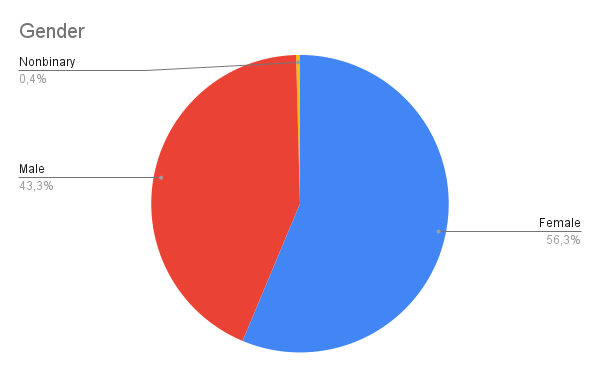
\includegraphics[width=15cm]{Images/General/03_user_centered_design/Survey/Gender.png}
    \caption{Chart showing the gender distribution of the survey participants}
    \label{fig:surveyGender}
\end{figure}
\FloatBarrier

La distribucion de las edades de las personas que respondieron, representada en el grafico \ref{fig:surveyAge}, muestra que se logro la meta propuesta de cubrir todas los grupos de edad posibles con la mayor cantidad de gente posible. Sin embargo tambien se puede ver claramente en la tabla \ref{tab:surveyAgeTable} que hay una gran discrepancia entre la cantidad de participantes por grupo de edad: El mas grande es el de los participantes entre los 60 y 69 anos con 84 participantes, seguido por el de los participantes entre los 18 y los 29 anos. Entre estos dos grupos hay una diferencia de tamano de aproximadamente 1.5. Esto hace que la media de edad suba un poco, a 47.88 anos, pero sigue siendo un valor medio en un rango aceptable, ya que la media de los participantes no es ni muy joven ni muy mayor, lo que comunica que el sample group que se alcanzo estuvo balanceado.

\FloatBarrier
\begin{figure}[!htbp]
    \centering
    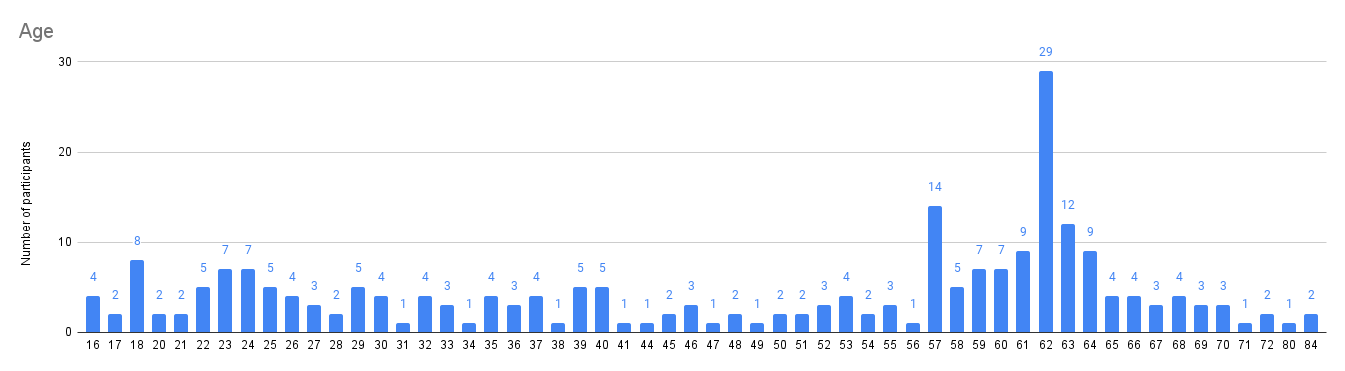
\includegraphics[width=15cm]{Images/General/03_user_centered_design/Survey/Age.png}
    \caption{Chart showing the age distribution of the survey participants}
    \label{fig:surveyAge}
\end{figure}
\FloatBarrier

\FloatBarrier
\begin{table}[!htbp]
    \centering
    \begin{adjustbox}{width=1\textwidth,center=\textwidth}
        \begin{tabular}{|c|c|c|c|c|c|c|c|}
        \hline
        15-18 & 18-29 & 30-39 & 40-49 & 50-59 & 60-69 & 70-79 & Age Average \\ \hline
        6 & 54 & 31 & 11 & 43 & 84 & 6 & 47,88 \\ \hline
        \end{tabular}
    \end{adjustbox}
    \caption{Table containing the participants per age group and the participant age average of the survey}
    \label{tab:surveyAgeTable}
\end{table}
\FloatBarrier

El utlimo punto demografico es el de las ocupaciones de los participantes (see \ref{fig:surveyOccupations}), donde se puede apreciar aun cuando "management occupations" y "Education, Training, and Library Occupations" tienen una cantidad considerable de participantes por detras, en general las otras ocupaciones tienen, aproximadamente, una distribución muy similar. Luego hay algunas ocupaciones mas fuera de lo comunes, como por ejemplo "Aviation" o "Behavioural health coach" , que previsiblemente, tienen una menor cantidad de participantes por detras. 

\FloatBarrier
\begin{figure}[!htbp]
    \centering
    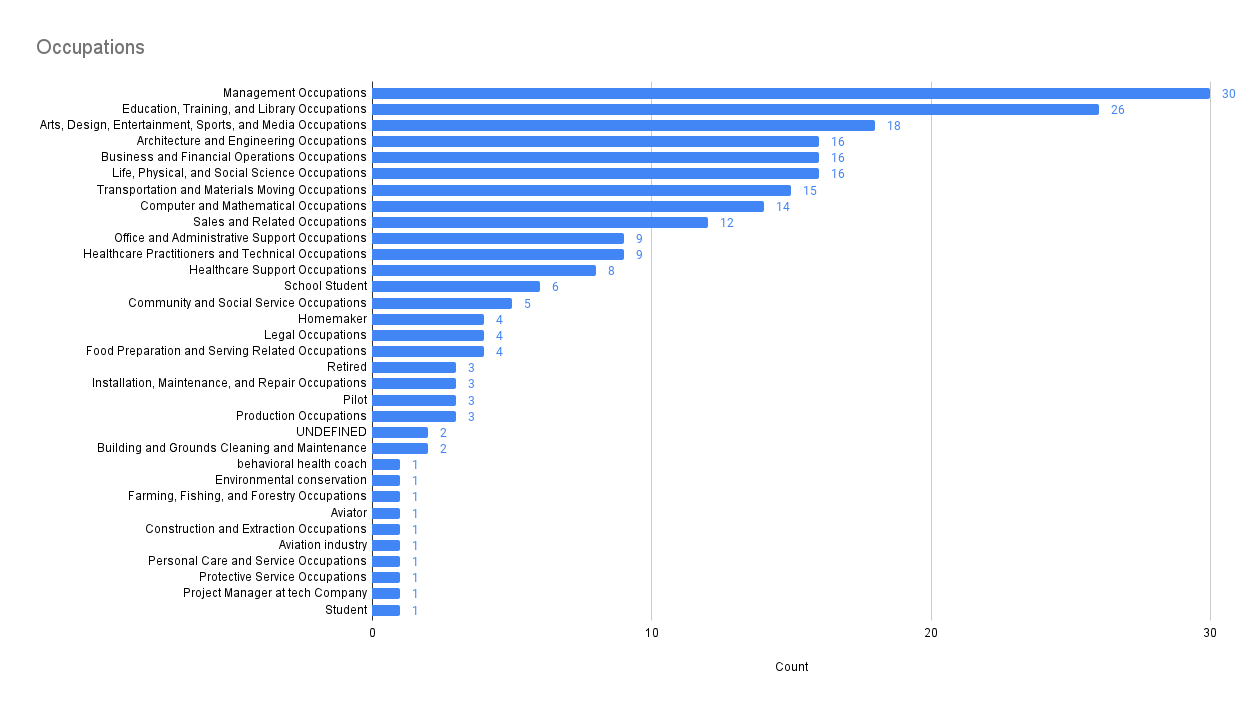
\includegraphics[width=15cm]{Images/General/03_user_centered_design/Survey/Occupations.png}
    \caption{Chart showing the occupations distribution of the survey participants}
    \label{fig:surveyOccupations}
\end{figure}
\FloatBarrier

Como se puede ver en \ref{fig:surveyTrackOrNot}, una gran mayoria de casi tres cuartos de los participantes mantenia algun tipo de registro, que no fuera mental, sobre sus tareas y actividades pendientes. Concretamente, esto quiere decir que de los 238 participantes 181 tenian un mecanismo establecido para tareas y 57 no.

\FloatBarrier
\begin{figure}[!htbp]
    \centering
    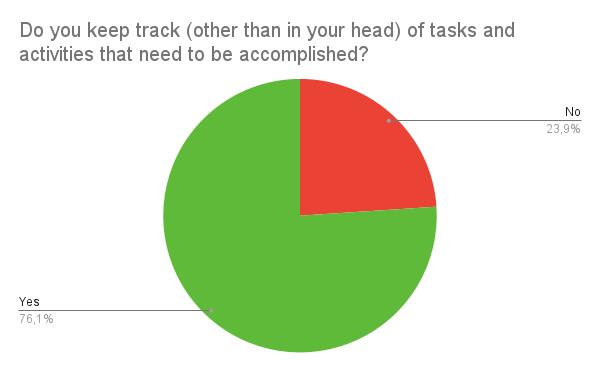
\includegraphics[width=15cm]{Images/General/03_user_centered_design/Survey/KeepTrack.png}
    \caption{Chart showing the distribution of participants that kept track of their pending tasks and participants that did not}
    \label{fig:survey}
\end{figure}
\FloatBarrier

En caso de que los participantes respondieran que no llevaban un registro de sus tareas pendientes, se les agradecia por haber participado en la encuesta y se terminaba esta, debido a que tenia poco sentido hacerles preguntas sobre un proceso que no tenian. En caso de que las respuesta fuera afirmativa se proseguia con las siguientes preguntas: 

\begin{enumerate}
    \item What do you use to keep track of your tasks and activities?
        \begin{enumerate}
            \item Paper (Any type and format)
            \item Digital
            \item Both
        \end{enumerate}
    \item Select all the digital tools you use to keep track of your tasks and activities.
        \begin{enumerate}
            \item None
            \item Digital calendar (e.g. Google Calendar, Apple Calendar, Microsoft Calendar, etc.)
            \item Notes application on your smartphone
            \item Simple text file (e.g. Word, Notepad, etc.)
            \item Application/Software that only allows the creation of checklists and offers basic functionalities such as reminders, categorization, etc. (e.g. Google Keep, AnyList, Checkvist, etc.).
            \item Application/Software that only allows the creation of checklists and offers advanced functionalities such as a calendar, collaboration with other people or other social functionalities, etc. (e.g. Todoist, Google Tasks, Amie, etc.).
            \item Project management software (e.g. Jira, Trello, Asana, etc.).
            \item Highly customizable general purpose app/software, which is software that has no structure and acts as a blank canvas where the user can choose from a large number of features to build the customized system they need (e.g. OneNote, Notion, etc.).
            \item Other...
        \end{enumerate}
    \item Select all the features that you regularly use when tracking your tasks and activities.
        \begin{enumerate}
            \item None
            \item Setting a date and/or time for a task or activity (Adding them to a calendar would also qualify)
            \item Use the priority of the tasks or activities to sort them (e.g. high priority items are done first)
            \item Any sort of categorization (color coding, different lists, flags, etc.)
            \item Set reminders or alarms for tasks or activities
            \item Add media (images, videos, etc.) or links
            \item Print out the created plan
            \item Share tasks with other people (email, social networks, instant messaging, etc.)
            \item Other...
        \end{enumerate}
    \item How do you usually write down your tasks and activities?
        \begin{enumerate}
            \item Using full and correct sentences
            \item Using key words or short sentences that may be grammatically or syntactically incorrect
        \end{enumerate}
    \item Roughly how many tasks and activities are currently in your list/calendar/etc.?
    \item Roughly how many of those tasks are from previous days or weeks and have been carried over to today?
    \item How satisfied are you with the personal system you have developed to track your tasks and activities?
    \item How satisfied are you with the tools (notebooks, software, etc.) you are currently using to track your tasks and activities?
\end{enumerate}

En este bloque estaban las ocho preguntas con las que se pretendia recopilar la informacion sobre las costumbres y rutinas de los participantes en cuanto a la organizacion de tareas pendientes. En este grupo habia dos preguntas de seleccion simple (1 y 4), dos preguntas de seleccion multiple (2 y 3), dos preguntas donde el participante debia introducir un numero (5 y 6) y dos preguntabas donde el participante debia evaluar su satisfaccion en una escala de likert (7 y 8).\\
\\
Con las primeras tres preguntas se buscaba validar los resultados de la focus group. Primero se busco examinar si al incrementar el sample group, la alta cantidad de participantes que utilizaba un approach hibrido para organizar tareas pendientes se mantenia, como era el caso de todos los participantes del focus group. En la segunda pregunta se presento la categorizacion explicada anteriormente en el capitulo "State of the art" \ref{sec:stateOfTheArt}, el cual se genero con la ayuda de los resultados del grupo de discusión y en la tercera pregunta se utilizaron los features mas populares y mas mencionados por los participantes de la focus group. Con esto se buscaba recolectar informacion sobre cuales tipos de herramientas eran las mas populares y luego mas especificamente cuales features dentro de estas herramientas eran los mas utilizados. Con esta informacion se pretendia definir en que direccion se debia mover el proyecto en el proximo paso y que tipos de herramientas y features eran los mas interesantes para los participantes. \\
\\
Como se puede apreciar en \ref{fig:surveyToolType}, una gran mayoria de los participantes reporto que utilizaban tanto herramientas digitales como algun tipo de formato en papel para mantener organizadas sus tareas pendientes, lo cual coincide con los findings del focus group. Luego, un grupo de aproximadamente un tercio del tamano utilizaba unicamente herramientas digitales y por ultimo aproximadamente un 10\% utilizaba unicamente formatos de papel.

\FloatBarrier
\begin{figure}[!htbp]
    \centering
    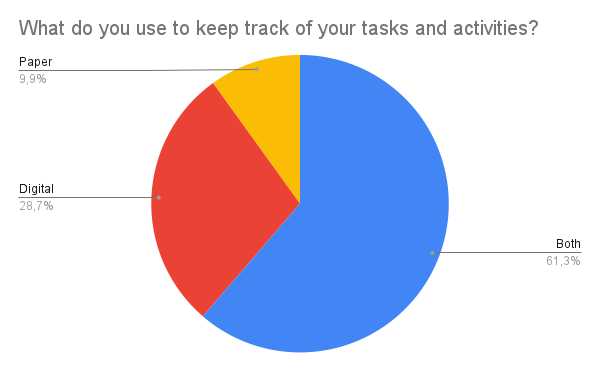
\includegraphics[width=10cm]{Images/General/03_user_centered_design/Survey/WhatKeepTrack.png}
    \caption{Chart showing the tools used by the survey participants}
    \label{fig:surveyToolType}
\end{figure}
\FloatBarrier

Luego, cuando se busco indagar mas concretamente en cuales herramientas digitales, los 181 participantes que si mantenian un registro de sus tareas pendientes proporcionaron 215 respuestas, por lo que era seleccion multiple (vea \ref{fig:surveyDigitalTools}). De las 215 respuestas se encontro que el calendario digital era, de lejos, la herramienta mas usada,  utilizado por 110 participantes o 51,2\%. Luego, con un gran margen, seguian my cerca uno del otro los documentos de texto simples y los enhanced task managers, utilizados por 25 (11,6\%) y 24 participantes (11,3\%), respectivamente. Estas herramientas fueron seguidas por los simple task managers, project management software y native note-taking apps, utilizadas respectivamente por 16 (7,4\%), 13 (6\%) y 12 (5,6\%) participantes. Los ultimos 15 votos (7,1\%) estaban principalmente divididos entre las highly customizable general purpose applications (3,3\%) y spreadsheets (2,8\%) y con un voto cada una (0,5\%), Salesforce and proprietary tools.

\FloatBarrier
\begin{figure}[!htbp]
    \centering
    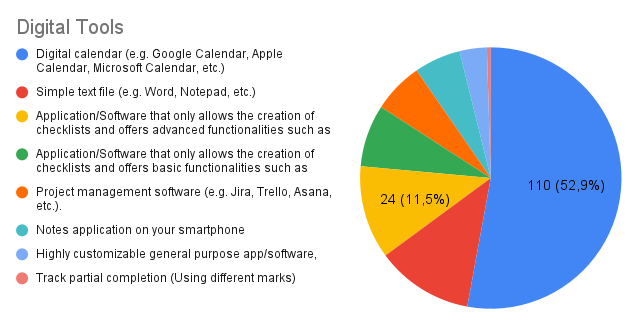
\includegraphics[width=10cm]{Images/General/03_user_centered_design/Survey/DigitalTools.png}
    \caption{Chart showing the digital tools used by the survey participants}
    \label{fig:surveyDigitalTools}
\end{figure}
\FloatBarrier

Por ultimo, al entrar en mas detalle sobre especificamente que features eran mayormente utilizados por los participantes, se encontro que los 4 features mas utilizados eran primero, y de nuevo de lejos, el poder agregar fecha y/o hora a una tarea, al por ejemplo, agregarla a un calendario, con 116 votos (46\%) de un total de 252, seguido por la utilizacion de reminders y alarmas, con 46 votos (18,3\%), cualquier tipo de categorizacion, con 34 votos (13,5\%) y poder agregar media (imagenes, videos, etc.) a una tarea, con 24 votos (9,5\%). Los ultimos 32 votos (12,8\%) fueron dados principalmente a la posibilidad de compartir tareas con otras personas (4,8\%), utilizar la prioridad de las tareas para organizarlas (4\%), imprimir el plan creado (3,6\%) y por ultimo el utilizamiento de diferentes simbolos para el seguimiento de la realización parcial de tareas (0,4\%).
%ADD REFLECTION TO FOCUS GROUP

\FloatBarrier
\begin{figure}[!htbp]
    \centering
    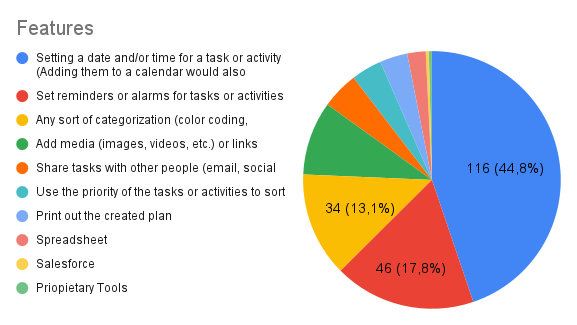
\includegraphics[width=10cm]{Images/General/03_user_centered_design/Survey/Features.png}
    \caption{Chart showing the features used by the survey participants}
    \label{fig:surveyFeatures}
\end{figure}
\FloatBarrier

Las preguntas 4, 5 y 6 fueron tomadas de un estudio realizado por ... en ..., donde buscaban ... Uno de los primeros pasos que realizaron para hacerse una idea sobre el campo y los habitos de la target population, fue hacer un snapshot study, donde entre otros, incluyeron estas tres preguntas. Debido a que el estudio fue realizado en ... y desde entonces la tecnologia se ha vuelto mas prevalecente en la vida diaria, especialmente notable en el area de los smartphone, se considero interesante incluir estas mismas preguntas no solo por el valor que traeria saber como y cuantas tareas manejaban los participantes en promedio, un valor que se puede utilizar cuando se considerara los tamanos y espacios para visualizar las tareas, sino tambien poder comparar ambos resultados y ver si han cambiado con el paso del tiempo.\\ Como se puede ver en \ref{fig:surveyWriteDown}, una vasta mayoria de los participantes (65,1\%) escribe sus tareas pendientes utilizando keywords u oraciones cortas en lugar de oraciones largas y correctas gramatical- o sintacticamente (35,9\%). 

\FloatBarrier
\begin{figure}[!htbp]
    \centering
    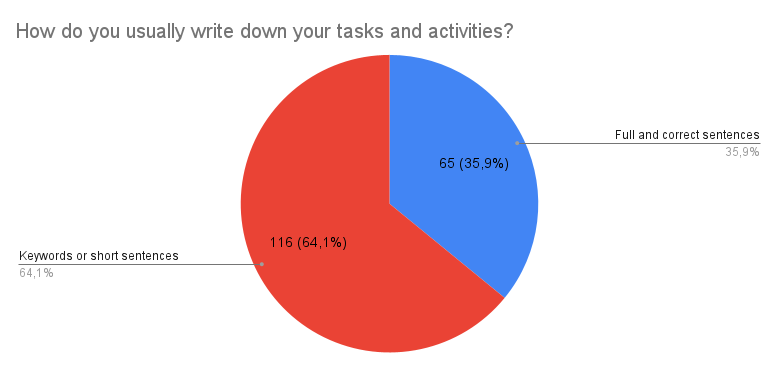
\includegraphics[width=10cm]{Images/General/03_user_centered_design/Survey/WriteDown.png}
    \caption{Chart showing how the participants usually wrote their pending tasks down.}
    \label{fig:surveyWriteDown}
\end{figure}
\FloatBarrier

Los participantes reportaron que tenian al momento de la encuesta, en promedio, una cantidad de 25 tareas pendientes anotadas, de las cuales, en promedio, 6,85 eran tareas de dias anteriores y que se habían traspasado debido a que no se habian cumplido.\\ 
\\
Las ultimas dos preguntas pedian al participante que calificaran su satisfaccion en cuanto a su sistema de organizacion de tareas pendientes y tambien en cuanto a las herramientas que utilizaban para esto. Esta informacion podia resultar util para medir si, en promedio, la gente estaba satisfecha o si estaban a la busqueda de algo mejor. Para valorar su satisfaccion se utilizo una escala de Likert, donde un extremo decia "Not satisfied at all, I need a better solution." y el otro "Completely satisfied, I wouldn't change anything.". La escala de Likert se utilizo debido a que al tener cinco posibles valoraciones, se ofrecia a los participantes valoraciones que iban desde lo extremadamente negativo a lo extremadamente positivo con una opcion neutral en el medio.\\
En promedio, el sentimiento de los participantes hacia sus sistemas actuales para organizar sus tareas pendientes y las herramientas que utilizaban eran ambos neutrales tendiendo a positivo, con una puntuacion de 3,8 y 3,91 respectivamente.


CON ESTE PASO se finalizo el proceso del analisis Comprender y describir el contexto de usousabilityUXBook 
%Trial added student bit
%A bit long answers but important they be clear in functionality and diferences
%Keine Nutzungsanforderungen spezifizieren (Konzeption)
\myparagraph{Findings}

\section{Paper prototype and heuristic evaluation}
%Rapid Prototype 
    %Focus on testing functionalities rather than UI
    %Some things left out on purpose to see results 
        %Information in the list vs. no information

The next step after having collected and evaluated information about different aspects of task tracking using the focus group and the survey was to start converting the collected knowledge into a concrete solution. Siguiendo el proceso del user centered design, antes de empezar con la implementacion de la aplicacion o de siquiera crear un prototipo digital, se diseno primero un prototipo de papel que involucrara la menor cantidad de esfuerzo, tiempo y recursos. El prototipo debia tener justo lo suficiente como para transmitir la idea general de la aplicacion y sus funcionalidades, para poder realizar con el una evaluacion heuristica. De esta manera se podian conseguir errores de usabilidad de manera rapida y economica y el feedback se podia directamente incluir en el prototipo digital y por extension, en la aplicacion.\\ 

\subsection{Prototypes}
Basado en la informacion recopilada se decidio crear tres prototipos, que en esencia eran muy similares entre si pero cada uno pretendia buscar una posible mejora o como minimo, ser un soporte para ayudar con una necesidad concreta. Los tres prototipos representan un enhanced task manager, debido a que no solo ofrecen funcionalidades basicas para organizar tareas sino que tambien buscan mejorar el proceso con funcionalidades avanzadas.

\subsubsection{Version 1}
La primera version del prototipo ofrecia diferentes funcionalidades que normalmente se pueden encontrar en aplicaciones para organizar las tareas pendientes. El prototipo ofrece tres visualizaciones diferentes: Una lista de tareas, un calendario y un editor de texto, los cuales son accesibles a traves de los tabs en la parte superior (vea \ref{}). En la barra superior tambien hay un toggle con el que se puede abrir o cerrar un side menu, un boton para volver a home y una barra de busqueda donde se pueden buscar tareas o categorias. En la parte superior del menu lateral se pueden observar las diferentes categorias que ha creado el usuario, en el medio se pueden ver dos botones con los que se pueden acceder diferentes funcionalidades del editor de texto, que seran explicadas con mayor detalle mas adelante y abajo el usuario puede acceder a su cuenta de usuario. En la lista de tareas el usuario puede ver sus tareas organizadas por categoria y puede filtrar las categorias visibles haciendo click en los nombres de las categorias en el menu lateral. El calendario ofrece las funcionalidades basicas donde el usuario puede agregar, visualizar y modificar tareas organizadas por fecha y hora (vea \ref{}).

%Add Gamification/Process tracking
%Numbered image
\begin{figure}
    \centering
    \includegraphics{}
    \caption{List View}
    \label{fig:my_label}
\end{figure}

\begin{figure}
    \centering
    \includegraphics{}
    \caption{Calendar View}
    \label{fig:my_label}
\end{figure}

Naturalmente, se puede hacer click en las tareas para editarlas, tanto en la lista como en el calendario, y se pueden agregar nuevas tareas haciendo click en el boton en la esquina inferior derecha. En ambos casos se abre una ventana (vea \ref{}) donde el usuario puede introducir el titulo de la tarea, agregar una descripcion o mas detalles sobre la tarea y puede asignar una fecha y hora, una categoria, una prioridad y reminders a la tarea. Ademas le puede asignar subtasks, que son tareas que son partes de la tarea que deben ser completados antes de poder completar la tarea.\\
La funcionalidad del editor de texto es lo que diferencia esta version de otros editores, debido a que no solo permite al usuario recolectar notas y pensamientos que pueda tener a lo largo del dia sino que tambien le permite agregar y organizar sus tareas en forma de texto, sin necesidad de interactuar con la interfaz o utilizar el mouse y dichas tareas son automaticamente visibles en la lista de tareas y el calendario. Para esto se pretende brindar al usuario una serie de shortcuts y opciones para formatear sus tareas de manera de que sean identificadas y guardadas automaticamente por la aplicacion. Las opciones son las siguientes: 

\begin{itemize}
    \item Starting a line with /t will add it as a task
    \item A date and time can be set by either writing them directly, e.g. 23/04/2022 13:30 or by using keyboards like /today, /tomorrow, etc.
    \item The task can be made recurring by adding /rec\_d for a daily repetition cycle or /rec\_w for a weekly cycle
    \item The priority of the task can be set by adding a flag ranging from /p1 to /p5
    \item The category can be set with the /<category> flag, where the category is either set if it already exists or created and set if it does not exist. 
    \item Sub-tasks can be added by following the same structure described previously and indenting the tasks to represent the hierarchy. 
\end{itemize}

El usuario tiene la opcion de acceder al editor de text con el tab superior o a traves del panel lateral, donde hay dos botones diferentes: "Today's notes" y "Tasks \& Notes". Estas dos opciones abren editores de texto que funcionan de igual manera pero que buscan visualizar diferentes tipos de contenido. "Today's notes" busca representar una especie de diario, donde todos los dias se genera automaticamente un documento de texto nuevo donde el usuario puede anotar todas las tareas, ideas y notas que tenga para ese dia. Ademas, las tareas que deba completar en el dia apareceran en la lista, aun si se han agregado en dias anteriores. Por el otro lado "Tasks \& Notes" es una coleccion general de notas y tareas, que no se borra ni se regenera de manera diaria. Contiene todas las tareas que el usuario ha recopilado en su lista de tareas y todas las notas que el usuario haya hecho previamente. La diferencia de acceder a la funcionalidad desde el menu lateral o utilizando el tab, es que el tab siempre abre un editor para "Today's notes" de ventana completo y si se abren las opciones desde el menu lateral, estas se abren como split screen on the bottom of the screen en cualquier visualizacion que el usuario tenga abierta en el momento. 

\subsubsection{Version 2}
La segunda version del prototipo contenia las mismas funcionalidades basicas presentadas en la primera version, pero en vez de tener un editor de texto ofrecia funcionalidades orientadas a visualizar y manejar las dependencias entre tareas. La primera diferencia se puede apreciar en la lista de tareas, donde cada tarea tiene un boton (vea \ref{}) con el que se pretende brindar al usuario la opcion de agregar nuevos sub-tasks sin tener que hacer click en la tarea y agregar el subtask en la nueva ventana. En cambio, al hacer click en este boton se abre una ventana (vea \ref{}) donde el usuario puede buscar, filtrar y elegir entre las tareas existentes o agregar una nueva. 

El calendario tambien presenta una gran diferencia ya que ofrece una barra de dependencias encima del calendario normal. Esta barra, que se puede expandir o colapsar, muestra para cada tarea que tenga una fecha limite, las sub-tasks que no se han completado y que deben ser completadas. Estas sub-tasks se visualizan en forma de barras que corren hasta el dia en que termina la tarea y pretenden servir como una representacion visual de cuanto tiempo le queda al usuario para completar dichas tareas. 

Por ultimo, esta version ofrece, la "card view", una visualizacion completamente nueva en lugar del editor de texto. Aqui los usuarios pueden ver todas sus tareas en forma de tarjeta, que contiene todos los subtasks de la tarea y esta coloreada dependiendo del estatus de los subtasks. Si todos los subtasks han sido completados y la tarea tambien, la tarjeta sera de color verde. Si todos los subtasks han sido completados, pero la tarea no se ha marcado como completada la tarjeta tendra el color rojo. Y por ultimo, si no todos los subtasks han sido completados la tarjeta no solo tendra el color rojo sino que tambien estara ligeramente greyed out.\\
Con esto se pretende ofrecer al usuario una rapida visualizacion del estatus de las sub-tasks de cada tarea. Si los sub-tasks de una tarea no han sido completados, la tarea principal no puede ser marcada como completada por lo que se presenta slightly greyed out. Una vez que todos los sub-tasks han sido completados es que se desbloquea esta tarea, perdiendo el color gris y se puede marcar como completa, cambiando el color de rojo a verde. 

\subsubsection{Version 3}
La tercera version del prototypo era una combinacion de los dos prototipos previamente descritos y se agrego principalmente para comprobar si el incluir todas las funcionalidades en una unica aplicacion seria demasiado abrumador para el usuario.

\subsection{Heuristic Evaluation}

\subsubsection{Procedure}
La evaluacion heuristica se llevo a cabo a traves de Zoom, para reducir el tiempo necesario para la organzacion y planeacion, con la ayuda de tres evaluadores. Segun Nielsen, 5/6 evaluadores expertos consiguen un 75\% de los problemas de usabilidad \ref{}, pero debido a los time constraints en este proyecto, se decidio reducirlo a tres.\\
Para la evaluacion se utilizaron las 10 heuristicas desarrolladas por Nielsen \ref{}. A los evaluadores se les explico que habia tres prototipos diferentes que debian evaluar solos y que el moderador solo intervendria en caso de que no supieran como proseguir o no entendieran nada. Debido a que era un prototipo de papel, la funcionalidad debia ser simulada por el moderador. Para esto se creo un board en Miro, donde se subieron todas las imagenes del prototipo y se armaron las diferentes ventanas. Debido a que el moderador podia ver la posicion del mouse del evaluador, este simplemente debia decir "right click" o "left click" y el moderador simularia lo que causaria ese click en la aplicacion real, moviendo y modificando las ventanas correctamente. Se les pidio a los evaluadores que realizaran dos pases, el primero para familiarisarze con la aplicacion y en el segundo para entrar mas en detalle y evaluar la interfaz y en caso de que consiguieran un problema de usabilidad debian anotarlo en una tabla que se les habia proporcionado. Alli debian brevemente describir el problema, donde ocurria, que heuristica violaba y le debian dar un indice de severidad. Para calcular este indice debian tomar en cuenta primero, que tan a menudo ocurria, que tanto afectaba el cumplimiento de la tarea y que tan facil era de evadir una vez que se sabia que existia dicho problema. Teniendo en cuenta estos criterios, se debia dar una puntuacion de 1 a 4 con las siguientes calificaciones: 

\begin{enumerate}
    \item \textbf{Cosmetic problem only:} No need to fix, unless extra time is available in the project
    \item \textbf{Minor usability problem:} fixing this should be given low priority
    \item \textbf{Major usability problem:} important to fix, so should be given high priority
    \item \textbf{Usability catastrophe:} imperative to fix this before the product can be released
\end{enumerate}

Una vez todos los expertos hubieran realizado una evaluacion, los resultados se resumieron y se enviaron por correo a cada evaluador los problemas descubiertos por los otros dos expertos, de manera que pudieran tambien darle una evaluacion de severidad. De esta manera se podia generar una media para calcular la severidad de todos los problemas y ordenarlos de mayor a menor severidad. Basado en este proceso se encontraron los problemas de usabilidad descritos en la proxima seccion.

\subsubsection{Findings}
The three evaluators found a combined sum of 47 usability issues, displayed in the table below \ref{tab:usabilityIssues}. La tabla está ordenada de manera descendente por la calificación media de la gravedad de las tareas y tiene informacion sobre en que version del prototipo fue conseguido el error, una breve descripcion del problema y donde ocurre, que heuristicas han sido violadas segun los diferentes participantes y por ultimo, las severity ratings que dio cada evaluador a los problemas y su average. \\
Cuando se les pidio a los evaluadores que calificaran los problemas encontrados por los otros evaluadores, unicamente se les pidio que dieran un severity rating, por lo que hay problemas que no tienen heuristicas para cada evaluador, solo para aquellos que notaron el problema durante la evaluacion. Por el otro lado, durante este paso salio a la luz que durante la primera evaluacion tanto al evaluador como al moderador se les paso evaluar en el prototipo dos el calendario y su barra de dependencias (vea \ref{fig:}). El prototipo de papel, como explicado anteriormente, tenia una gran cantidad de features y ventanas, las cuales debian ser movidas a mano a su sitio, como es usual con este tipo de prototipo. Al ser una evaluacion sin una estructura ni un proceso fijo, donde el orden de los pasos dentro de cada version los definian los usuarios. Esto, combinado con la inexperiencia, resultaron en que durante la primera evaluacion no se evaluara un feature tan importante como lo era la barra de dependencias sobre el calendario en la segunda version. Por este motivo, todas los problemas relacionados con este feature no tienen ninguna puntuacion por parte del primer evaluador y son solo el average de las puntuaciones de los otros dos evaluadores. Para combatir esto, se genero para las dos evaluaciones restantes un documento general que contenia todos los features que se debian analizar y, aun si era en otro orden, servia como guia para evitar olvidar evaluar un feature.\\
En cuanto a los resultados concretos, hubo 7 problemas que fueron evaluados con un average mayor a tres, de los cuales tres eran en relacion al primer prototipo. Primero, para los evaluadores no estuvo claro que habia una coneccion entre los botones en el menu lateral "Today’s Notes” y “Tasks & Notes" y el editor de texto

\FloatBarrier
\begin{table}[!htbp]
    \centering
    \resizebox{\textwidth}{!}{%
        \begin{tabular}{|l|l|l|l|l|l|l|l|l|l|l|l|}
             \hline
            \multirow{2}{*}{ Eval. } & \multirow{2}{*}{ Vers. } & \multirow{2}{*}{ Describe the issue } & \multirow{2}{*}{ Where/How does it occur? } & \multicolumn{3}{c}{Violated Heuristic} & \multicolumn{5}{c}{Severity } \\ \hline
            & & & & Eval. 1 & Eval. 2 & Eval. 3 & Eval. 1 & Eval. 2 & Eval. 3 & AVG. & AVG (Num) \\ \hline
            1 & 1 & It is not clear that the buttons “Today’s Notes” and “Tasks & Notes” refer to the text editor and functionality. The link between these two aspects should be clearer, e.g., by adding a “Text” title to the sidebar. & Sidebar -> Today’s Notes and Tasks & Notes & 4 & & & 4 & 4 & 3 & 3.7 & 3.67 \\ \hline
            1 & 1 & The functionality of the notification system and how notifications should be configured correctly, is not clear. & “Add/Edit Task” Window -> Notifications & 2 & & 6 & 3 & 4 & 3 & 3.3 & 3.33 \\ \hline
            2 & 1,2,3 & The calendar has no navigation to move forwards or backwards between weeks and months, making it impossible for the user to select any other week or month. & Calendar View & & 3 & 3 & 3 & 4 & 3 & 3.3 & 3.33 \\ \hline
            1 & 1 & The meaning of the “Today’s Notes” and “Tasks & Notes” buttons/icons in the side menu is not clear. & Sidebar -> Today’s Notes and Tasks & Notes & 6 & & & 4 & 2 & 3 & 3.0 & 3.00 \\ \hline
            2 & 2 & If a week has many tasks, which in turn also have many subtasks, the dependency bar in the calendar will become very crowded and confusing.
            A way to reduce this, could be by highlighting the subtasks in the bar and graying out other subtasks when hovering with the mouse over a task in the calendar. & Dependency Calendar View & & 6, 7, 5 & & & 4 & 2 & 3.0 & 3.00 \\ \hline
            3 & 1 & There is no way of closing the text editor split screen window, e.g. with an x on the top left corner. & Split Screen Text Editor & & & 3 & 3 & 3 & 3 & 3.0 & 3.00 \\ \hline
            3 & 2 & The tag icon in the “Add subtask” dialogue does not convey the fact that it is supposed to be used to filter the list. & Dependency List View -> “Add subtask” dialogue & & & 1,2 & 3 & 3 & 3 & 3.0 & 3.00 \\ \hline
            1 & 1 & Wrong text in the button when editing a task instead of adding a new one, as it should say “Save Task” instead of “Add Task” & “Add/Edit Task” Window & 2 & & 4 & 2 & 3 & 3 & 2.7 & 2.67 \\ \hline
            1 & 1 & There is no way of setting the duration of a task. There is only one field to set a time. & “Add/Edit Task” Window
            -> Calendar & 11 & & & 2 & 3 & 3 & 2.7 & 2.67 \\ \hline
            1 & 2 & Having to click on each subtask and the parent task to complete them is cumbersome and annoying. The main task should be completed when all subtasks are completed. & “Dependencies” view & 7 & & & 2 & 4 & 2 & 2.7 & 2.67 \\ \hline
            2 & 1 & The click-to-edit functionality of the tasks in the “list” view is not clear. When hovering over a task with the mouse, an edit icon should appear. This would also improve keyboard support. & “List View” & & 10, 3 & & 2 & 4 & 2 & 2.7 & 2.67 \\ \hline
            2 & 1 & There are too many, very specific commands in the text editor which the users have to memorize. & Text View & & 6 & & 1 & 4 & 3 & 2.7 & 2.67 \\ \hline
            3 & 1 & It is not clear how the tasks should be built in the text editor.
            Should the commands be placed before, after, in a specific order, etc.? & Text Editor & & & 1 & 2 & 3 & 3 & 2.7 & 2.67 \\ \hline
            3 & 1 & There are no examples or step by step guides on how a task should be defined in the text editor.
            The first time, a short step by step guide could be shown to the user. & Text Editor & & & 10 & 3 & 3 & 2 & 2.7 & 2.67 \\ \hline
            3 & 1 & The list provides no information about the task other than the title and category.
            The user needs to click each task to gather more information about it. & List view & & & 6 & 3 & 2 & 3 & 2.7 & 2.67 \\ \hline
            3 & 2 & The meaning of the dependency icon in the list view is not clear. & Dependency List View -> Dependency Button & & & 1,2 & 2 & 3 & 3 & 2.7 & 2.67 \\ \hline
            3 & 2 & To avoid possible errors, the user should not be able to cross-out/complete tasks in the “Add Subtask” dialogue, as this is not a feature the user would expect in this dialogue. & Dependency List View -> “Add subtask” dialogue & & & 5 & 2 & 3 & 3 & 2.7 & 2.67 \\ \hline
            3 & 2 & Completed tasks should be placed at the bottom of the list and incomplete tasks at the top. & General & & & 8 & 3 & 3 & 2 & 2.7 & 2.67 \\ \hline
            3 & 2 & The subtasks in the dependency bar should only reach up to the beginning of their due day, as reaching the middle of the day could falsely indicate that the user has half a day more than they actually have. & Dependency Calendar -> Dependency Bar & & & 1 & & 4 & 1 & 2.5 & 2.50 \\ \hline
            3 & 2 & The icon to open and close the dependency bar can be mistaken with a drag & drop to resize the window. & Dependency Calendar -> Dependency Bar & & & 4 & & 3 & 2 & 2.5 & 2.50 \\ \hline
            3 & 2 & The dependency bar over the calendar offers no way of crossing-out/completing the subtasks. & Dependency Calendar -> Dependency Bar & & & 4 & & 3 & 2 & 2.5 & 2.50 \\ \hline
            1 & 1 & To access the edit functionality of the “Today’s Notes” and the “Task & Notes” buttons on the sidebar, the user has to click twice (right click and then “Edit”), which presents a context menu with just two menu items.
            This can be avoided by, for example, showing the icons when hovering over with the mouse. & Sidebar -> Today’s Notes and Tasks & Notes & 7 & & & 2 & 3 & 2 & 2.3 & 2.33 \\ \hline
            1 & 1 & Meaning and difference between the terms “Task” and “Notes” is not clear. & General & 2 & & & 3 & 2 & 2 & 2.3 & 2.33 \\ \hline
            1 & 1 & The category buttons on the sidebar do not clearly show that they are interactable and that by clicking them, the list can be filtered. A filter icon or label is missing. & Sidebar -> Category List & 4 & & 1 & 2 & 4 & 1 & 2.3 & 2.33 \\ \hline
            1 & 2 & It is not clear what a grayed-out task means in the dependency view. & “Dependencies” view & 11 & & & 2 & 4 & 1 & 2.3 & 2.33 \\ \hline
            1 & 1,2,3 & The home button does not conform with expectations as it is not clear what home means in this context. It is also made redundant by the tab system.
            The home or default view should be displayed directly on the tabs. For example, by adding a small home icon to the home tab. & Top navigation bar & 8 & & & 1 & 4 & 2 & 2.3 & 2.33 \\ \hline
            1 & 3 & Too many tabs and functionalities, which makes the system overwhelming. Set the focus on less but better thought out views. & General, Top navigation bar & 8 & & & 2 & 4 & 1 & 2.3 & 2.33 \\ \hline
            2 & 1 & There are no labels or placeholders in input fields in the “Add/Edit Task” window. This makes it unclear, which makes it unclear what the fields are for. & “Add/Edit Task” Window & & 1, 3, 6 & & 2 & 4 & 1 & 2.3 & 2.33 \\ \hline
            2 & 1,2,3 & Empty states (previously explained), should be used all over the application so that it is always clear to the user when “emptiness” is caused by an error or is actually intended. & General & & 1, 3, 6, & & 2 & 4 & 1 & 2.3 & 2.33 \\ \hline
            2 & 2 & The dependency cards should allow for a quick way of adding subtasks, e.g. by providing an input field directly below the existing subtasks. This allows the user to work more quickly and saves clicks. & Dependency View & & 3 & & 2 & 3 & 2 & 2.3 & 2.33 \\ \hline
            2 & 2 & The subtasks and dependencies between the tasks are not directly visible in the list view. To view the subtasks, the user needs to click on each task to open a different window. There is no way of viewing a task’s parent task. & List View & & 3,5 & & 3 & 2 & 2 & 2.3 & 2.33 \\ \hline
            3 & 1 & The tutorial of the text editor contains too much text and is overwhelming. The sentences should be shortened. & Text Editor -> Tutorial & & & 6, 10 & 2 & 4 & 1 & 2.3 & 2.33 \\ \hline
            3 & 1 & The tutorial has no explicit way of closing it, e.g. with an x on the corner. & Text Editor -> Tutorial & & & 3 & 2 & 3 & 2 & 2.3 & 2.33 \\ \hline
            3 & 2 & There is no way of sorting the cards in the dependency view, e.g. by completion, by time of creation, etc. & Dependency View & & & 7 & 2 & 3 & 2 & 2.3 & 2.33 \\ \hline
            1 & 1 & No visible marker or signal to indicate which tab is currently selected. Needs to be visually highlighted and connected to the current selection. & Top Navigation Bar -> Tabs & 1 & & & 2 & 3 & 1 & 2.0 & 2.00 \\ \hline
            1 & 1 & The “List” view does not show the relationship between tasks and their subtasks (e.g. by indenting the subtasks under their parent) & List view & 1 & & & 2 & 2 & 2 & 2.0 & 2.00 \\ \hline
            1 & 1 & The meaning of the flag icon is not clear. Can be confused with the meaning on other platforms, where it is used to flag/report content or issues. & “Add/Edit Task” Window & 4 & & & 2 & 2 & 2 & 2.0 & 2.00 \\ \hline
            1 & 1 & The priorities have no color coding (from green to red), which would help the user to recognize the severity of each priority. & “Add/Edit Task” Window -> Priorities & 6 & & & 3 & 2 & 1 & 2.0 & 2.00 \\ \hline
            2 & 1 & When the text editor is opened, the focus should be automatically placed in the input field. This way the user can start typing right away, saving unnecessary clicks and making the experience smoother. & Text Editor & & 1 & 1, 6 & 2 & 2 & 2 & 2.0 & 2.00 \\ \hline
            2 & 2 & If the dependency bar in the calendar view is closed, the information about the amount of subtasks that a task has, is not visible. The user would need to open the dependency bar each time and look for the subtasks.
            This can be avoided by adding the amount of subtasks to the event in the calendar. & Dependency Calendar View & & 6, 7 & & & 2 & 2 & 2.0 & 2.00 \\ \hline
            3 & 1 & The term “indenting” is not clear to everyone. & Text Editor -> Tutorial & & & 2 & 1 & 3 & 2 & 2.0 & 2.00 \\ \hline
            3 & 2 & The task cards (not the subtasks) in the dependency view have no way of being crossed-out/completed. & Dependency View & & & 4 & 2 & 2 & 2 & 2.0 & 2.00 \\ \hline
            1 & 1 & The meaning of the tag icon is not clear, as it is not used anywhere else. It does not immediately transmit that it is supposed to represent the categories. & “Add/Edit Task” Window & 4 & & & 1 & 2 & 2 & 1.7 & 1.67 \\ \hline
            2 & 1,2,3 & When a task has no subtasks an empty state should be used. Empty states explicitly tell the user, that the fact that they are not seeing any content is intended. This way the user can differentiate between empty lists caused by an error of the application and empty lists caused by the lack of content.
            An example of this would be to move the title and the add button to the middle and use a dashed line for the outline. & “Add/Edit Task” Window -> Subtasks
            
            
            Exam. of ”empty state” & & 1 & & 2 & 2 & 1 & 1.7 & 1.67 \\ \hline
            2 & 1,2,3 & The title “Subtasks” and the “Add” button are too close to each other, which makes the button seem more like an icon rather than a button. This could be solved by placing the button on the right side of the container & “Add/Edit Task” Window -> Subtasks & & 6 & & 2 & 2 & 1 & 1.7 & 1.67 \\ \hline
            2 & 1 & The buttons in the side menu “Today’s Notes” and “Tasks & Notes” open a window on the bottom of the screen. Placing them on the side menu creates a mental distance for the user, making the behavior of opening a window on the bottom of the screen unexpected. Placing the buttons on the bottom of the screen makes the behavior more predictable. & Sidebar -> Today’s Notes and Tasks & Sidebar -> Today’s Notes and Tasks & Notes & & 5, 6 & 1,2 & 2 & 2 & 1 & 1.7 & 1.67 \\ \hline
            3 & 2 & Completed tasks should be cleared after a specified timeframe, e.g. daily, weekly, etc.. & General & & & 8 & 2 & 2 & 1 & 1.7 & 1.67 \\ \hline
        \end{tabular}}
    \caption{Usability issues found during the heuristic evaluation}
    \label{tab:usabilityIssues}
\end{table}
\FloatBarrier
        
\section{Digital Prototype}
El prototipo general se desarrollo basado en los resultados de la evaluacion del prototipo.